% !TEX TS-program = pdflatex
% Shifa --- codebase-derived technical description (thesis-style, expanded).
% Build: pdflatex SHIFA_SYSTEM_TECHNICAL_DESCRIPTION.tex (run twice for TOC).
% Requires: MiKTeX/TeX Live with TikZ (pgf).

% Use openany to avoid blank "openright" pages in digital PDFs.
\documentclass[11pt,a4paper,twoside,openany,headings=normal]{scrreprt}

% Page geometry (submission-grade margins)
\usepackage[a4paper,left=3cm,right=2.5cm,top=2.5cm,bottom=2.5cm]{geometry}

\usepackage[utf8]{inputenc}
\usepackage[T1]{fontenc}
\usepackage{lmodern}
\usepackage{microtype}
\usepackage{setspace}
\usepackage{xurl}
\usepackage[none]{hyphenat} % Disable hyphenation across the document.
\usepackage[hidelinks,pdfusetitle]{hyperref}
\usepackage{enumitem}
\usepackage{booktabs}
\usepackage{longtable}
\usepackage{array}
\usepackage{tabularx}
\usepackage{graphicx}
\usepackage{amssymb}
\usepackage{float}
\usepackage{ragged2e}
\usepackage{caption}

\usepackage{tikz}
\usetikzlibrary{positioning,arrows.meta,calc,backgrounds,shapes.geometric}

\usepackage{pdfpages}

% TikZ figures included from SHIFA_SYSTEM_TECHNICAL_DESCRIPTION.tex
% Requires: \usepackage{tikz}, positioning, arrows.meta, shapes.geometric, calc, backgrounds, fit

\newcommand{\ShifaFigSystemContext}{%
\begin{figure}[!htbp]
\centering
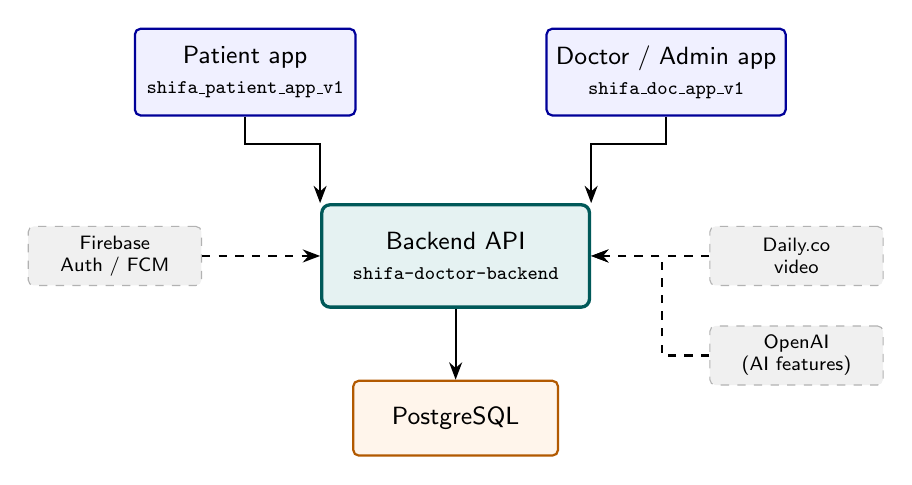
\begin{tikzpicture}[
  font=\small\sffamily,
  node distance=6mm and 10mm,
  client/.style={rounded corners=2pt, draw=blue!60!black, thick, fill=blue!6, minimum width=2.8cm, minimum height=1.1cm, align=center},
  core/.style={rounded corners=3pt, draw=teal!70!black, very thick, fill=teal!10, minimum width=3.4cm, minimum height=1.3cm, align=center},
  data/.style={rounded corners=2pt, draw=orange!70!black, thick, fill=orange!8, minimum width=2.6cm, minimum height=0.95cm, align=center},
  ext/.style={rounded corners=2pt, draw=gray!60, dashed, fill=gray!12, minimum width=2.2cm, minimum height=0.75cm, align=center, font=\scriptsize\sffamily},
  arr/.style={-{Stealth[length=2.2mm]}, thick}
]
\node[client] (p) {Patient app\\\scriptsize\texttt{shifa\_patient\_app\_v1}};
\node[client, right=2.4cm of p] (d) {Doctor / Admin app\\\scriptsize\texttt{shifa\_doc\_app\_v1}};
\path (p.south) -- coordinate[midway] (midtop) (d.south);
\node[core, below=1.1cm of midtop] (api) {Backend API\\\scriptsize\texttt{shifa-doctor-backend}};
\node[data, below=0.9cm of api] (db) {PostgreSQL};
\node[ext, left=1.5cm of api] (fb) {Firebase\\Auth / FCM};
\node[ext, right=1.5cm of api] (daily) {Daily.co\\video};
\node[ext, below=0.5cm of daily] (ai) {OpenAI\\(AI features)};
\draw[arr] (p.south) -- ++(0,-0.35) -| (api.north west);
\draw[arr] (d.south) -- ++(0,-0.35) -| (api.north east);
\draw[arr] (api) -- (db);
\draw[arr, dashed] (fb.east) -- (api.west);
\draw[arr, dashed] (daily.west) -- (api.east);
\draw[arr, dashed] (ai.west) -- ++(-0.6,0) |- (api.east);
\end{tikzpicture}
\caption{High-level system context: two Flutter clients, one Spring Boot API, PostgreSQL, and main external integrations.}
\label{fig:system-context}
\end{figure}%
}

\newcommand{\ShifaFigPatientNav}{%
\begin{figure}[!htbp]
\centering
\begin{tikzpicture}[
  font=\small\sffamily,
  tab/.style={rounded corners, draw, minimum width=1.85cm, minimum height=0.65cm, align=center},
  shell/.style={rounded corners, draw=teal!60, thick, inner sep=6pt},
  lbl/.style={font=\scriptsize\itshape}
]
\node[shell, label=above:\textbf{StatefulShellRoute (indexedStack)}] (ss) {
\begin{tikzpicture}[node distance=3mm]
\node[tab, fill=teal!10] (h) {Home};
\node[tab, fill=teal!10, right=of h] (b) {Bookings};
\node[tab, fill=teal!10, right=of b] (doc) {Docs};
\node[tab, fill=teal!10, right=of doc] (dr) {Doctors};
\end{tikzpicture}};
\node[shell, below=8mm of ss, label=above:\textbf{ShellRoute + bottom bar}] (sh) {
\begin{tikzpicture}[node distance=3mm]
\node[tab, fill=gray!15] (a) {Account};
\node[tab, fill=gray!15, right=of a] (c) {Chat};
\node[tab, fill=gray!15, right=of c] (n) {Notif.};
\node[tab, fill=gray!15, right=of n] (t) {Tasks};
\end{tikzpicture}};
\node[tab, fill=red!12, dashed, thick, below=8mm of sh, minimum width=6cm] (v) {Video call (fullscreen, no bottom bar)};
\node[lbl, left=2mm of ss.west, align=right] {GoRouter};
\end{tikzpicture}
\caption{Patient app navigation: four primary tabs preserve state per branch; account/chat/notifications/tasks share another shell; video is outside shells.}
\label{fig:patient-nav}
\end{figure}%
}

\newcommand{\ShifaFigDoctorShell}{%
\begin{figure}[!htbp]
\centering
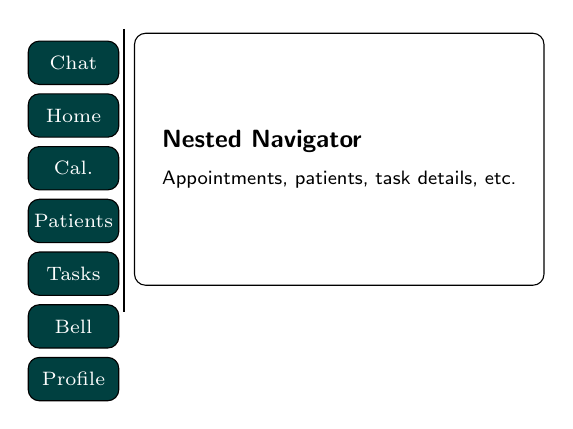
\begin{tikzpicture}[
  font=\small\sffamily,
  sb/.style={rounded corners, draw, fill=teal!50!black, text=white, minimum width=1.15cm, minimum height=0.55cm, inner sep=2pt, font=\scriptsize},
  main/.style={draw, rounded corners, minimum width=5.2cm, minimum height=3.2cm, align=left, inner sep=8pt}
]
\node[sb, anchor=north west] (n0) at (0,0) {Chat};
\node[sb, below=3pt of n0.south west, anchor=north west] (n1) {Home};
\node[sb, below=3pt of n1.south west, anchor=north west] (n2) {Cal.};
\node[sb, below=3pt of n2.south west, anchor=north west] (n3) {Patients};
\node[sb, below=3pt of n3.south west, anchor=north west] (n4) {Tasks};
\node[sb, below=3pt of n4.south west, anchor=north west] (n5) {Bell};
\node[sb, below=3pt of n5.south west, anchor=north west] (n6) {Profile};
\node[main, anchor=north west, xshift=1.35cm, yshift=0.1cm] (content) at (0,0) {\textbf{Nested Navigator}\\[0.25em]
\scriptsize Appointments, patients, task details, etc.};
\draw[thick] (1.22,0.15) -- (1.22,-3.45);
\end{tikzpicture}
\caption{Doctor \texttt{MainShell}: vertical sidebar (schematic) and inner \texttt{Navigator} for stacked routes.}
\label{fig:doctor-shell}
\end{figure}%
}

\newcommand{\ShifaFigBackendLayers}{%
\begin{figure}[!htbp]
\centering
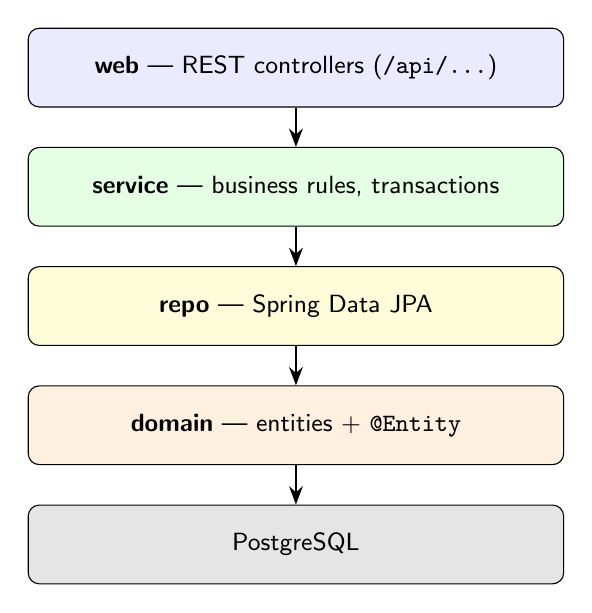
\begin{tikzpicture}[
  font=\small\sffamily,
  layer/.style={rounded corners, draw, minimum width=6.8cm, minimum height=1.0cm, align=center},
  arr/.style={-{Stealth}, thick}
]
\node[layer, fill=blue!8] (w) {\textbf{web} --- REST controllers (\texttt{/api/...})};
\node[layer, fill=green!10, below=5mm of w] (s) {\textbf{service} --- business rules, transactions};
\node[layer, fill=yellow!15, below=5mm of s] (r) {\textbf{repo} --- Spring Data JPA};
\node[layer, fill=orange!12, below=5mm of r] (d) {\textbf{domain} --- entities + \texttt{@Entity}};
\node[layer, fill=gray!20, below=5mm of d] (db) {PostgreSQL};
\draw[arr] (w) -- (s);
\draw[arr] (s) -- (r);
\draw[arr] (r) -- (d);
\draw[arr] (d) -- (db);
\end{tikzpicture}
\caption{Backend layering in \texttt{com.shifa}: controllers delegate to services, repositories, and JPA entities.}
\label{fig:backend-layers}
\end{figure}%
}

\newcommand{\ShifaFigJwtFlow}{%
\begin{figure}[!htbp]
\centering
\resizebox{\textwidth}{!}{%
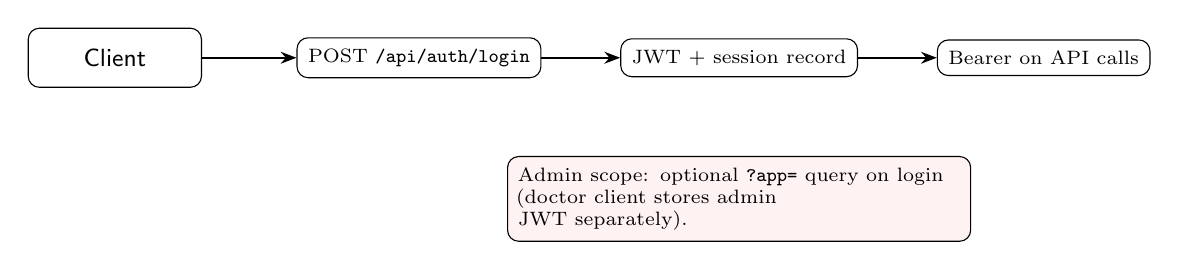
\begin{tikzpicture}[
  font=\small\sffamily,
  scale=0.94,
  actor/.style={rounded corners, draw, minimum height=0.75cm, minimum width=2.2cm, align=center},
  jwtbox/.style={rectangle, draw, rounded corners, inner sep=4pt, align=center, font=\scriptsize},
  arr/.style={-{Stealth[length=2mm]}, thick}
]
\node[actor] (c) {Client};
\node[jwtbox, right=1.2cm of c] (a) {POST \texttt{/api/auth/login}};
\node[jwtbox, right=1.0cm of a] (j) {JWT + session record};
\node[jwtbox, right=1.0cm of j] (r) {Bearer on API calls};
\draw[arr] (c) -- (a);
\draw[arr] (a) -- (j);
\draw[arr] (j) -- (r);
\node[jwtbox, below=1.0cm of j, text width=5.6cm, align=left, fill=red!5] (note) {Admin scope: optional \texttt{?app=} query on login\\(doctor client stores admin\\JWT separately).};
\end{tikzpicture}%
}
\caption{Simplified authentication flow\\
(see \texttt{AuthController},\\
\texttt{JwtAuthFilter}).}
\label{fig:jwt-flow}
\end{figure}%
}

\newcommand{\ShifaFigSecurityRisk}{%
\begin{figure}[!htbp]
\centering
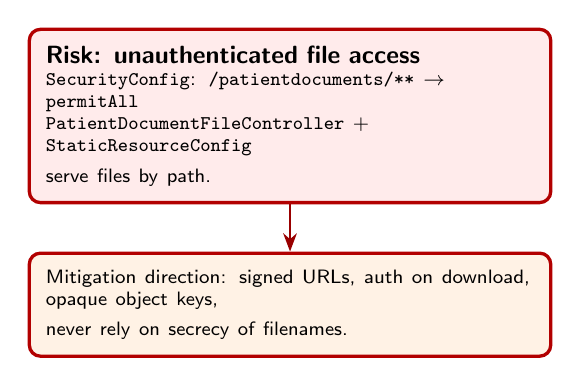
\begin{tikzpicture}[
  font=\small\sffamily,
  bad/.style={rounded corners, draw=red!70!black, very thick, fill=red!8, align=left, text width=6.2cm, inner sep=6pt},
  arr/.style={-{Stealth}, thick, red!60!black}
]
\node[bad] (box) {
\textbf{Risk: unauthenticated file access}\\
\scriptsize\texttt{SecurityConfig}: \texttt{/patientdocuments/**} $\rightarrow$ \texttt{permitAll}\\
\scriptsize\texttt{PatientDocumentFileController} + \texttt{StaticResourceConfig}\\serve files by path.};
\node[bad, below=6mm of box, fill=orange!10] (mit) {\scriptsize Mitigation direction: signed URLs, auth on download, opaque object keys,\\never rely on secrecy of filenames.};
\draw[arr] (box) -- (mit);
\end{tikzpicture}
\caption{Document URL exposure (code-derived): treat as high severity until redesigned.}
\label{fig:security-risk}
\end{figure}%
}

\newcommand{\ShifaFigDeployment}{%
\begin{figure}[!htbp]
\centering
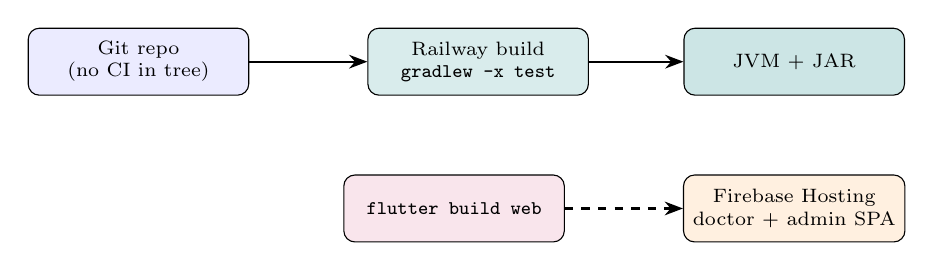
\begin{tikzpicture}[
  font=\small\sffamily,
  box/.style={rounded corners, draw, minimum width=2.8cm, minimum height=0.85cm, align=center, font=\scriptsize},
  arr/.style={-{Stealth}, thick}
]
\node[box, fill=blue!8] (gh) {Git repo\\(no CI in tree)};
\node[box, fill=teal!15, right=1.5cm of gh] (rw) {Railway build\\\texttt{gradlew -x test}};
\node[box, fill=teal!20, right=1.2cm of rw] (jar) {JVM + JAR};
\node[box, fill=orange!12, below=1.0cm of jar] (fb) {Firebase Hosting\\doctor + admin SPA};
\node[box, fill=purple!10, left=1.5cm of fb] (flt) {\texttt{flutter build web}};
\draw[arr] (gh) -- (rw);
\draw[arr] (rw) -- (jar);
\draw[arr, dashed] (flt) -- (fb);
\end{tikzpicture}
\caption{Deployment signals from repository files: backend ships via Railway-style Gradle build; doctor web via Flutter then Firebase Hosting.}
\label{fig:deployment}
\end{figure}%
}

\newcommand{\ShifaFigTestBars}{%
\begin{figure}[!htbp]
\centering
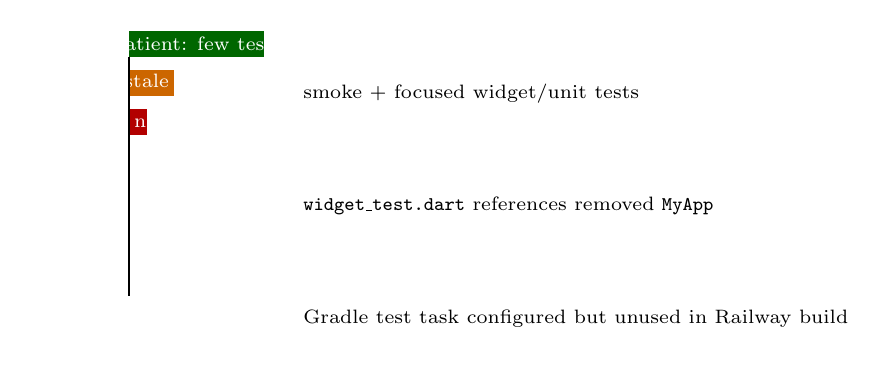
\begin{tikzpicture}[
  font=\small\sffamily,
  scale=0.95
]
\begin{scope}[x=0.12cm,y=0.35cm]
\fill[green!40!black] (0,0) rectangle (15,1) node[midway, text=white, font=\scriptsize] {Patient: few tests};
\fill[orange!80!black] (0,-1.5) rectangle (5, -0.5) node[midway, text=white, font=\scriptsize] {Doctor: stale template};
\fill[red!70!black] (0,-3) rectangle (2, -2) node[midway, text=white, font=\scriptsize] {Backend: no src/test};
\end{scope}
\draw[thick] (0,0) -- (0,-3.2);
\node[anchor=west, font=\scriptsize] at (2.2,-0.5) {smoke + focused widget/unit tests};
\node[anchor=west, font=\scriptsize] at (2.2,-2) {\texttt{widget\_test.dart} references removed \texttt{MyApp}};
\node[anchor=west, font=\scriptsize] at (2.2,-3.5) {Gradle test task configured but unused in Railway build};
\end{tikzpicture}
\caption{Qualitative automated test coverage as inferred from repository structure (not line coverage).}
\label{fig:test-bars}
\end{figure}%
}


% Allow PDF includes with newer PDF versions (must be set in preamble).
\pdfminorversion=7

% Consistent formatting for technical strings (paths, filenames, routes).
% Use \codepath{...} to ensure stable monospace without letterspacing artifacts.
\newcommand{\codepath}[1]{\texttt{\detokenize{#1}}}
\let\path\codepath

\title{Technical Description of the Shifa System\\[0.5em]
\large A Codebase-Derived Architectural Document (Patient App, Doctor App, Backend)}
\author{Compiled from repository sources}
\date{\today}

\hypersetup{
  pdftitle={Shifa System Technical Description},
  pdfauthor={Shifa repositories}
}

\begin{document}

% --- Global typography & layout (thesis-style consistency) ---
\onehalfspacing

% Paragraph policy (thesis-grade): first-line indent, no extra vertical gap.
\setlength{\parindent}{0.5cm}
\setlength{\parskip}{0pt}

% Lists: consistent indentation, spacing, and wrapped-line alignment.
\setlist[itemize]{leftmargin=*,align=parleft,itemsep=0.25\baselineskip,topsep=0.25\baselineskip,parsep=0pt}
\setlist[enumerate]{leftmargin=*,align=parleft,itemsep=0.25\baselineskip,topsep=0.25\baselineskip,parsep=0pt}

% Figures/tables: consistent caption style and float spacing.
\captionsetup{font=small,labelfont=bf,justification=RaggedRight,singlelinecheck=false,width=\linewidth}
\setlength{\intextsep}{0.8\baselineskip}
\setlength{\textfloatsep}{1.0\baselineskip}
\setlength{\floatsep}{0.8\baselineskip}

% Hyphenation: reduce aggressive word breaking (esp. TOC).
\pretolerance=1000
\tolerance=2000
\emergencystretch=2em
\hbadness=20000
\vbadness=20000
\hyphenpenalty=10000
\exhyphenpenalty=10000

% TOC: reduce ugly hyphenation.
\sloppy

% Standardize heading spacing (KOMA-Script)
\RedeclareSectionCommand[beforeskip=1.6\baselineskip,afterskip=0.8\baselineskip]{chapter}
\RedeclareSectionCommand[beforeskip=1.2\baselineskip,afterskip=0.6\baselineskip]{section}

% Replace the LaTeX title cover with the Word-exported cover page.
% This ensures the first cover page matches your Word thesis.

\includepdf[pages={1},pagecommand={}]{theory_part.docx_export.pdf}

\chapter*{Deutsche Zusammenfassung}
\addcontentsline{toc}{chapter}{Deutsche Zusammenfassung}

Diese Masterarbeit untersucht die Entwicklung und prototypische Umsetzung einer Telemedizin-Plattform (Shifa) für den usbekischen Versorgungskontext. Ausgangspunkt sind qualitative Befunde aus ärztlichen Interviews, die wiederkehrende Probleme in der Versorgungspraxis sichtbar machen: informelle und fragmentierte Kommunikation, manuelle Terminorganisation, uneinheitliche Dokumentation, Risiken von Datenverlust sowie Unsicherheit in rechtlich sensiblen Situationen.

Auf dieser Grundlage werden funktionale und technische Anforderungen systematisch abgeleitet und in eine implementierbare Architektur überführt. Die Lösung umfasst zwei Client-Anwendungen (Patient und Arzt/Admin), ein zentrales Backend mit rollenbasierter Zugriffskontrolle sowie persistente Datenhaltung in PostgreSQL. Ergänzend werden externe Dienste für OTP-basierte Authentifizierung, Benachrichtigungen und Videokonsultationen eingebunden.

Die Arbeit zeigt damit die Nachvollziehbarkeit des Übergangs von empirisch erhobenen Bedarfen zu konkreten Architektur- und Implementierungsentscheidungen. Gleichzeitig werden Grenzen des aktuellen Prototyps transparent ausgewiesen, insbesondere in Bezug auf produktionsreife Absicherung, Betriebsreife und vollständige Vertragsformalierung der APIs.

\chapter*{English Abstract}
\addcontentsline{toc}{chapter}{English Abstract}

This Master's thesis investigates the design and prototype implementation of a telemedicine platform (Shifa) for the healthcare context of Uzbekistan. The work is grounded in qualitative physician findings that indicate recurring delivery problems, including informal and fragmented communication, manual appointment coordination, discontinuous documentation practices, exposure to data-loss risks, and legal uncertainty in remote-care settings.

Based on these findings, the thesis derives functional and technical requirements and translates them into an implementable system architecture. The resulting prototype consists of two client applications (patient and doctor/admin), a central backend with role-aware access control, and PostgreSQL-based persistence. External services are integrated for OTP-oriented authentication, notifications, and video consultation workflows.

The contribution of the thesis is the traceable link between empirical needs and concrete implementation decisions. At the same time, the document explicitly reports prototype boundaries, especially regarding production-grade hardening, operational maturity, and fully formalized API contracts.

\chapter*{Acknowledgements}
\addcontentsline{toc}{chapter}{Acknowledgements}

I would like to express my sincere gratitude to my supervisors for their guidance, critical feedback, and continuous support throughout this thesis project. Their academic advice helped shape both the research framing and the technical implementation.

I also thank all participating physicians and users who contributed their time and practical insights. Their perspectives were essential for grounding this work in real clinical and operational needs.

My appreciation further goes to my family and friends for their encouragement and patience during the development and writing phases.

\clearpage

\tableofcontents
\listoffigures
\listoftables

\chapter{Background, Problem Statement and Objectives}

\section{Background and Rationale}\label{background-and-rationale}

Uzbekistan's health system, like those of many post-Soviet states, has
undergone a complex and protracted reform process since independence in
1991. The legacy of the Semashko model - characterized by centralized
planning, public financing and provision, and a strong hospital sector -
has shaped both the strengths and persistent challenges of the system.
Over the past three decades, the country has sought to replace
input-driven norms with outcomes-focused governance, strengthen primary
health care (PHC), and reduce out-of-pocket (OOP) payments that threaten
financial protection and equity. (Ketevan Glonti, 2013)

Despite important gains - particularly in routine immunization, maternal
and child health, and the introduction of strategic purchasing pilots -
Uzbekistan continues to face high OOP payments, gaps in financial
protection, underdeveloped quality assurance, and pronounced
rural--urban disparities. The burden of non-communicable diseases (NCDs)
has risen sharply, with ischemic heart disease, stroke, and cancers now
the leading causes of mortality. These epidemiological pressures,
combined with infrastructure and workforce constraints, have exposed the
limitations of traditional, hospital-centric models and underscored the
need for innovative, data-driven, and patient-centered approaches.
(World Health Organization, 2022)

In this context, digital health, including telemedicine platforms,
electronic health records, and e-referral systems---has emerged as a
promising instrument for health system improvement. The government's
``Concept on Health Development 2019--2025'' and subsequent strategies
have prioritized digitalization as a lever for expanding access,
improving quality, and enhancing efficiency. Early pilots in Syrdarya
region, including telemedicine clinics, e-referral systems, and digital
queue management, represent a notable inflection point in the country's
reform trajectory. (World Health Organization, 2022)

However, the digital health agenda is nascent and faces significant
barriers: legacy paper-based systems, fragmented data flows, uneven
facility readiness, limited digital literacy, and the absence of robust
governance and interoperability standards. Against this backdrop, this
thesis offers an integrated theoretical examination of health system
transformation in Uzbekistan, anchored in the specificities of the Uzbek
case and informed by comparative regional and international experience.

\section{Problem Statement and Research Questions}\label{problem-statement-and-research-questions}

\textbf{Problem Statement:}

Uzbekistan's health system faces persistent challenges in healthcare
access, service efficiency, and equity - particularly in rural areas and
among vulnerable populations. Despite ongoing reforms and digital health
pilots, gaps remain in infrastructure, coordination, and responsiveness.
Telemedicine platforms offer a promising solution, but their design must
be grounded in the lived experiences and needs of both patients and
healthcare providers. This thesis investigates how a telemedicine
platform can be developed and tested to address these challenges, based
on direct input from users and providers within the Uzbek health system.

\textbf{Research Questions:}

\begin{itemize}
\item
  What are the main barriers to healthcare access as perceived by
  patients in Uzbekistan, and how can digital tools address these
  barriers?
\item
  What are the key service delivery inefficiencies experienced by
  doctors, and what features would improve their workflow and patient
  management through a telemedicine platform?
\item
  What functional and technical requirements should a telemedicine
  platform meet to be usable, acceptable, and effective for both
  patients and providers in Uzbekistan?
\item
  How do users (patients and doctors) respond to a prototype
  telemedicine platform, and what does their feedback reveal about its
  potential to improve access and efficiency?
\end{itemize}

\section{Objectives of the Thesis}\label{objectives-of-the-thesis}

\begin{itemize}
\item
  To identify key barriers to healthcare access and service delivery
  efficiency in Uzbekistan through empirical surveys of patients and
  healthcare providers.
\item
  To translate user-reported challenges into functional and technical
  requirements for a telemedicine platform tailored to Uzbekistan's
  health system context.
\item
  To design and develop a prototype digital portal for patients and
  doctors that addresses the identified needs and supports improved
  access and workflow efficiency.
\item
  To evaluate the usability, acceptability, and perceived effectiveness
  of the telemedicine platform through pilot testing with real users.
\item
  To contribute to the theoretical and practical understanding of
  user-centered digital health design in post-Soviet health systems
  undergoing reform.
\end{itemize}


\chapter{Historical Background, Key Challenges and Health Outcomes}

Healthcare System in Uzbekistan

\section{Historical Background and Current Organization}\label{historical-background-and-current-organization}

Uzbekistan's health system is a product of its Soviet legacy, shaped by
the Semashko model---a highly centralized, state-funded, and
state-delivered system emphasizing hospital-based care, vertical disease
programs, and quantitative targets for inputs such as beds and staff
(Bernd Rechel M. A., 2014). During the Soviet era, health care was
nominally free at the point of use, with a focus on communicable disease
control, maternal and child health, and the expansion of physical
infrastructure. However, the system was characterized by inefficiencies,
underfunding, and a neglect of primary care and quality assurance (Bernd
Rechel E. R., 2014).

Following independence in 1991, Uzbekistan faced the dual challenge of
economic transition and health system reform. The early 1990s saw a
sharp contraction in public spending, a decline in health indicators,
and the emergence of informal payments and private provision (Bernd
Rechel M. A., 2014). The government responded with a series of reforms
aimed at rationalizing hospital capacity, strengthening PHC, and
introducing new financing mechanisms.

\textbf{Key Reform Milestones:}

\begin{itemize}
\item
  \textbf{1996 Law on Health Protection:} Established the legal basis
  for a state-guaranteed benefits package, including primary care,
  emergency care, and care for ``socially significant and hazardous''
  conditions (Bernd Rechel M. A., 2014).
\item
  \textbf{1998 Presidential Decree:} Launched a state program for health
  system reform, prioritizing PHC, emergency care, and the development
  of the private sector (Bernd Rechel M. A., 2014).
\item
  \textbf{2000s--2010s:} Implementation of World Bank and ADB-supported
  projects (Health I, II, III; Woman and Child Health Development)
  focused on PHC infrastructure, maternal and child health, and
  financing reforms (Bernd Rechel M. A., 2014). (The World Bank, 2025)
\item
  \textbf{2018--2021:} Adoption of the ``Concept on Health Development
  2019--2025'' (Presidential Decree 5590), establishment of the SHIF,
  and piloting of strategic purchasing and digital health initiatives in
  Syrdarya (The World Bank, 2025).
\end{itemize}

\textbf{Current Organization:}

The health system is organized into three administrative tiers:

\begin{itemize}
\item
  \textbf{National (Republican) Level:} Ministry of Health, national
  research institutes, tertiary hospitals, and regulatory agencies.
\item
  \textbf{Regional (Viloyat) Level:} Regional health authorities,
  multi-specialty hospitals, and specialized centers.
\item
  \textbf{District/City Level:} District medical unions, central
  hospitals, family polyclinics, and rural physician points (Bernd
  Rechel M. A., 2014).
\end{itemize}

The MoH remains the principal steward, with direct management of
national-level institutions and regulatory oversight of regional and
district facilities. The private sector, while growing, is still limited
in scope and subject to strict licensing and regulatory controls (The
World Bank, 2025).

\textbf{Service Delivery Model:}

\begin{itemize}
\item
  \textbf{Primary Care:} Delivered through family doctor points,
  polyclinics, and rural physician posts. PHC reforms have aimed to
  shift from specialist-dominated polyclinics to generalist-led family
  medicine, but progress has been uneven (Bernd Rechel A. S., 2023).
\item
  \textbf{Secondary and Tertiary Care:} Provided by district, regional,
  and national hospitals, with a legacy of overcapacity and
  fragmentation. Recent reforms aim to consolidate specialized centers
  into multi-specialty general hospitals (The World Bank, 2025)
\item
  \textbf{Emergency Care:} A well-developed network of emergency
  departments often better equipped than other public facilities, but
  subject to overload due to gaps in PHC and benefits coverage (World
  Health Organization, 2022).
\end{itemize}

\textbf{Governance and Regulation:}

Regulation is highly centralized, with the MoH and Cabinet of Ministers
responsible for policy, financing, and oversight. Local authorities have
limited autonomy, and dual accountability structures persist (Bernd
Rechel M. A., 2014). The regulatory framework for private providers and
pharmaceuticals is evolving, with recent efforts to strengthen
licensing, quality assurance, and market surveillance (The World Bank,
2025).

\section{Key Challenges in Access, Quality, and Financing}\label{key-challenges-in-access-quality-and-financing}

\textbf{Access:}

Despite improvements in health indicators, access to quality care
remains uneven. Rural-urban disparities are pronounced, with rural areas
facing shortages of qualified staff, inadequate infrastructure, and
limited access to diagnostics and medicines (Bernd Rechel A. S., 2023).
For example, only 57\% of PHC facilities reported basic water services
and 26\% basic sanitation in 2020, reflecting broader readiness
constraints (World Health Organization, 2022).

Geographical access is further constrained by the distribution of
facilities and workforce. While the number of physicians per 100,000
population has increased to 276 by 2019, and nurse density to
\textasciitilde1,100 per 100,000, these resources are concentrated in
urban centers. Outward migration of health professionals, especially to
Russia and Kazakhstan, exacerbates shortages in underserved areas.
(Bernd Rechel E. R., 2014)

\textbf{Quality:}

Quality of care is undermined by several factors:

\begin{itemize}
\item
  \textbf{Legacy of Input-Based Planning:} The Soviet system prioritized
  quantitative targets (beds, staff) over outcomes, with limited
  attention to quality assurance, patient safety, or evidence-based
  practice (Ketevan Glonti, 2013).
\item
  \textbf{Outdated Clinical Protocols:} Many facilities rely on outdated
  or poorly adapted clinical guidelines, with limited adoption of
  international best practices (Bernd Rechel M. A., 2014).
\item
  \textbf{Weak Monitoring and Evaluation:} Data systems are fragmented,
  paper-based, and focused on structural indicators rather than process
  or outcome measures. Quality improvement initiatives are limited in
  scope and sustainability (The World Bank, 2025)
\item
  \textbf{Patient Experience:} User experience is often neglected, with
  long waiting times, limited appointment systems, and a lack of
  patient-centered care models (Bernd Rechel M. A., 2014).
\end{itemize}

\textbf{Financing:}

The health financing system is characterized by:

\begin{itemize}
\item
  \textbf{Low Public Spending:} Public spending on health was
  \textasciitilde2.3\% of GDP in 2019, above the Central Asia average
  but well below the WHO European Region average (\textasciitilde5\%)
  (World Health Organization, 2022).
\item
  \textbf{High Out-of-Pocket Payments:} OOP payments accounted for
  57.7\% of current health expenditure in 2019, exposing households to
  financial hardship and catastrophic health spending. In 2020, 18\% of
  households reported cost-related nonuse of care (World Health
  Organization, 2022)
\item
  \textbf{Fragmented Pooling and Purchasing:} Budgeting is historically
  incremental, with limited strategic purchasing or risk pooling. The
  SHIF pilot in Syrdarya aims to introduce capitation and DRG-based
  payments, but implementation is nascent and faces capacity constraints
  (The World Bank, 2025).
\item
  \textbf{Limited Benefits Coverage:} The basic benefits package covers
  primary and emergency care, but excludes much of secondary/tertiary
  care and outpatient medicines, amplifying OOP and incentivizing
  emergency use (The World Bank, 2025).
\end{itemize}

\textbf{Equity and Financial Protection} (Bernd Rechel M. A.,
2014)\textbf{:}

\begin{itemize}
\item
  \textbf{Vulnerable Groups:} While the benefits package includes
  provisions for vulnerable groups (e.g., children, pregnant women,
  people with disabilities), eligibility criteria are not directly
  linked to income, and coverage gaps persist.
\item
  \textbf{Informal Payments:} Informal payments remain widespread,
  particularly in secondary and tertiary care, undermining equity and
  trust in the system.
\end{itemize}

\section{Health Outcomes and Risk Profile}\label{health-outcomes-and-risk-profile}

\textbf{Demographic and Epidemiological Trends} (WHO Regional Office for
Europe, 2023)\textbf{:}

\begin{itemize}
\item
  \textbf{Population:} 33.3 million in 2020, with a young age structure
  but a growing burden of NCDs.
\item
  \textbf{Life Expectancy:} Increased from 67.2 years in 2000 to 73.9
  years in 2016, with a gender gap of 4.7 years.
\item
  \textbf{Maternal and Infant Mortality:} Maternal mortality declined
  from 41 per 100,000 live births in 2000 to 29 in 2017; infant
  mortality from 51.8 per 1,000 in 2000 to 15.6 in 2019.
\item
  \textbf{NCDs:} Account for 84\% of all deaths in 2018, with ischemic
  heart disease and stroke as leading causes.
\item
  \textbf{Risk Factors:} High systolic blood pressure (30.7\%), dietary
  risks (28.2\%), and high fasting plasma glucose (20.2\%) are dominant
  contributors to mortality.
\end{itemize}

\textbf{Service Coverage and UHC Index} (World Health Organization,
2022)\textbf{:}

\begin{itemize}
\item
  \textbf{UHC Service Coverage Index:} Improved from 56 (2000) to 71
  (2019), below OECD/EU comparators but signaling progress.
\item
  \textbf{Immunization:} High coverage rates for childhood vaccines, but
  challenges remain in TB, HIV/AIDS, and MDR-TB.
\end{itemize}

\textbf{Social Determinants} (The World Bank Group, 2021)\textbf{:}

\begin{itemize}
\item
  \textbf{Poverty:} Poverty headcount ratio declined from 14.1\% in 2013
  to 11.4\% in 2018, but disparities persist.
\item
  \textbf{Water and Sanitation:} Infrastructure needs extensive
  rehabilitation, with poor access in many areas.
\end{itemize}


\chapter{Introduction, Health Context and Digital Health as a Systemic Enabler}

Digitalization \& Internet Infrastructure

\section{Introduction: Digital Health as a Systemic Enabler}\label{introduction-digital-health-as-a-systemic-enabler}

Digital transformation is now recognized as a foundational enabler of
health system reform, not merely a technical add-on. In Uzbekistan, the
digital health agenda is explicitly linked to the broader goals of
universal health coverage (UHC), equity, efficiency, and quality
improvement. The government's ``Digital Uzbekistan 2030'' strategy and
the National Health System Strategy 2030 both position digitalization as
a cross-cutting priority, aiming to create robust governance structures,
integrated platforms, and the necessary broadband and ICT infrastructure
to support health system modernization. (The World Bank, 2025)

However, the digital health landscape in Uzbekistan is shaped by the
legacy of Soviet-era information systems, the rapid but uneven expansion
of internet and mobile technologies, and persistent gaps in digital
literacy and organizational readiness. This section provides a
comprehensive analysis of the current state, challenges, and
opportunities for digitalization and internet infrastructure in
Uzbekistan's health sector.

\section[Post-2016 Reforms: Infrastructure, Connectivity, and Policy]{Post-2016 Reforms: Infrastructure, Connectivity, and Policy (The World Bank, 2025)}\label{post-2016-reforms-infrastructure-connectivity-and-policy-the-world-bank-2025}

Since 2016, Uzbekistan has embarked on an ambitious digital
transformation agenda, with health as a priority sector. The ``Digital
Uzbekistan 2030'' strategy sets out to strengthen digital governance,
create integrated information systems, and expand broadband connectivity
across the country. The National Health System Strategy 2030 further
articulates the role of digital health as a driver of system-wide
reform, emphasizing the need for interoperable platforms, data-driven
decision-making, and patient empowerment.

By 2023, up to 81\% of public medical organizations' legal entities had
been provided with internet connectivity. However, the quality and
reliability of internet access vary significantly, especially in rural
areas. The phased installation of local area networks (LANs) in
healthcare facilities is ongoing. Despite these advances, more than 50\%
of public medical organizations still lack LANs beyond administrative
offices, and the estimated need for computers ranges from 30,000 to
65,000 units.

The lack of adequate ICT infrastructure is a critical bottleneck for
digital health. Many facilities are underequipped, with insufficient
computers, outdated hardware, and no dedicated ICT maintenance staff.
The absence of robust data centers further limits the scalability of
national digital health systems.

\section{National and Local Health Information Systems}\label{national-and-local-health-information-systems}

Uzbekistan's health sector is characterized by a proliferation of more
than 35 unconnected nationwide IT e-health systems. These systems
operate in silos, with no integration or common master data usage among
Ministry of Health (MoH) information systems. There is no national
patient registry, no unified registry of healthcare providers, and no
standardized nomenclature or classifiers. As a result, integration of IT
systems across facilities is not feasible, and data exchange is severely
constrained. (WHO Regional Office for Europe, 2023)

At the facility level, only a limited number of organizations use
Patient Administration Systems (PAS), Electronic Medical Records (EMR),
or Hospital Information Systems (HIS). Under MoH initiatives, two
PAS/EMR systems have been piloted in Syrdarya region, and about five
local PAS/HIS vendors provide services to public and private clinics and
hospitals. However, these systems are not interoperable, and most
medical records remain paper-based, scattered across facilities, and
inaccessible for longitudinal patient care. (The World Bank, 2025)

\section{Digital Literacy and Adoption Rates (WHO Regional Office for Europe, 2023)}\label{digital-literacy-and-adoption-rates-who-regional-office-for-europe-2023}

Digital literacy among health professionals is highly variable. While
younger staff and those in urban centers are increasingly proficient
with computers and digital tools, many older providers lack basic ICT
skills. Continuous IT training is not yet institutionalized, and there
is no national strategy for digital capacity building in the health
workforce. This gap is compounded by the lack of standardized digital
workflows and the persistence of paper-based documentation, which
consumes significant provider time and undermines efficiency.

Patient digital literacy is also uneven, with urban populations more
likely to use digital health services than rural residents. The absence
of a national patient portal or unified engagement platform limits
opportunities for patients to access their health records, book
appointments, or participate in their care. Where electronic booking
systems exist, their use is limited and not widely spread. As a result,
patients are not ``in the driver's seat'' of their health journey, and
digital health remains largely provider-centric.

The success of digital health initiatives depends not only on technical
infrastructure but also on organizational readiness and change
management. In Uzbekistan, digitalization planning and management are
currently centralized within the MoH and its IT-focused company,
UZINFOCOM. There is no independent body tasked with overseeing digital
health development, and the process is often non-transparent to external
stakeholders, including hospitals, clinics, professional associations,
and patient groups. This lack of inclusive governance hinders buy-in and
slows the pace of digital transformation. (The World Bank, 2025)



\chapter{Qualitative Analysis of Doctors’ Perspectives on Telemedicine in Uzbekistan}

\section{Introduction}

This chapter presents a qualitative analysis of physicians’ perspectives on telemedicine in Uzbekistan. The aim is to identify practical challenges in current healthcare delivery and to derive functional and technical requirements for a telemedicine platform. The analysis builds on the research objectives outlined in Chapters 1.1--1.3 and addresses the following research question: How do doctors in Uzbekistan perceive, use, and evaluate telemedicine in routine practice, and what actionable requirements for a telemedicine platform can be derived from their experiences?

\section{Methodology}

The empirical basis of this study consists of fifteen semi-structured interviews conducted with physicians from Uzbekistan. The participants were selected using purposive sampling to ensure diversity in both geographic distribution and medical specialization. The sample includes physicians from regions such as Tashkent, Samarkand, Bukhara, Khorezm, Karakalpakstan (Nukus), Jizzakh, Kashkadarya, Surkhandarya, and Navoi, as well as from different specialties including general practice, cardiology, obstetrics and gynecology, pediatrics, and surgery. Participants were recruited through professional networks and direct outreach via email and messaging platforms. The selection aimed to capture a broad range of experiences with telemedicine across urban, semi-urban, and rural healthcare settings.

Each interview followed a structured guide consisting of seven thematic blocks: General Use and Attitudes, Video Calls, Appointment Scheduling, Data Collection and Management, Communication via Applications, Recording and Summarization, and Legal and Data Protection Aspects. Table~\ref{tab:mayring-survey-questions} summarizes the interview questions by category and descriptive label.

The analysis was conducted using qualitative content analysis following the approach proposed by Mayring (Mayring P., 2015). This method combines deductive and inductive category development in a systematic and transparent manner. In the first step, deductive main categories were defined based on the interview guide. Subsequently, inductive subcategories were developed through iterative analysis of the interview material. This involved paraphrasing, summarizing, and generalizing relevant text passages. The coding unit was defined as a sentence or a meaningful clause, while the context unit corresponded to the thematic interview blocks. All text segments were systematically assigned to categories based on predefined coding rules; multiple coding was permitted where statements addressed more than one thematic dimension.

During the analysis, categories were continuously refined to improve clarity and reduce overlap. Inclusion and exclusion criteria were defined for each category and supported by representative anchor quotes. The results were synthesized descriptively and analytically, including frequency-based observations where appropriate. A complete codebook, including category definitions and anchor examples, is provided in Appendix A. The full interview transcripts were translated into English and are documented separately in anonymized form.

\subsection{Complementary incorporation of patient perspectives}

The primary derivation of system requirements in this thesis is intentionally physician-centered. This choice follows from the role of physicians as workflow owners and clinical decision-makers in day-to-day care delivery, especially for appointment logic, documentation responsibilities, and risk-sensitive communication processes. Consequently, the requirement synthesis presented in Chapter~5 is anchored first in doctor interviews and subsequently reconciled with the implemented system architecture.

At the same time, patient perspectives were incorporated through two complementary channels. First, an exploratory assessment addressed access-related barriers and everyday digital habits relevant to telemedicine use. In methodological terms, this input is treated as problem-space evidence that supports triangulation and helps prioritize physician-derived requirements in relation to practical adoption constraints. It is not used for statistical generalization, nor as an independent basis for defining the core requirement set.

Second, patient perspectives are being integrated through ongoing prototype evaluation that focuses on usability, trust, and perceived impact during interaction with the developed applications. This evaluation is positioned as design- and acceptability-oriented evidence and is reported in the chapters that discuss implementation and user-interface realization. The following results section therefore concentrates on the physician interview corpus as the principal analytical source for the qualitative findings in this chapter.

\begin{longtable}{@{}l>{\RaggedRight\arraybackslash}p{0.62\textwidth}>{\RaggedRight\arraybackslash}p{0.20\textwidth}@{}}
\caption{Survey Questions by Category and Descriptive Label}\label{tab:mayring-survey-questions}\\
\toprule
Category & Question & Descriptive label \\
\midrule
\endfirsthead
\toprule
Category & Question & Descriptive label \\
\midrule
\endhead
\midrule
\multicolumn{3}{r@{}}{Continued on next page}\\
\endfoot
\bottomrule
\endlastfoot
A & Which telemedicine functions do you currently use in your practice? & Current telemedicine use \\
A & How has your daily work changed through telemedicine? & Impact on daily workflow \\
A & What expectations did you have of telemedicine before using it? & Initial expectations \\
A & How has your attitude toward telemedicine developed over time? & Attitude development over time \\
B & How often do you conduct videocalls with patients? & Frequency of videocalls \\
B & For what purposes do you mainly use videocalls? & Purpose of videocalls \\
B & What advantages do you see in using videocalls? & Perceived advantages \\
B & What challenges or problems occur during videocalls? & Challenges and problems \\
B & Are there patient groups for whom videocalls are particularly suitable or unsuitable? & Suitability by patient group \\
B & How do you assess the quality of medical care via videocall? & Quality of care via videocall \\
C & Do you use digital tools for appointment scheduling? If yes, which ones? & Use of digital appointment tools \\
C & How do you assess the acceptance of digital appointment scheduling among your patients? & Patient acceptance \\
C & What advantages and disadvantages do you see in digital appointment scheduling? & Pros and cons of digital scheduling \\
C & Were there technical or organizational problems when introducing digital appointment scheduling? & Implementation problems \\
D & How do you collect and store patient data digitally? & Digital data collection methods \\
D & Which systems or apps do you use for data exchange? & Systems for data exchange \\
D & How do you assess the security and reliability of these systems? & Data security and reliability \\
D & What advantages and risks do you see in digital data exchange and storage? & Advantages and risks of digital data \\
D & Have you ever experienced problems with data loss or data security? & Experience with data issues \\
D & How do you handle documentation and archiving of digital data? & Data documentation and archiving \\
E & Do you communicate with patients through special apps? If yes, how? & App communication with patients \\
E & Do you communicate with other doctors via digital platforms or apps? & App communication with colleagues \\
E & Which functions are most important to you in app communication (e.g., security, speed, documentation)? & Important app features \\
E & What challenges exist in digital communication with patients and colleagues? & Challenges in app communication \\
F & Do you use functions for automatic recording or summarization of videocalls? & Use of recording \\
F & How useful would such recording functions be for your work? & Usefulness of recording tools \\
F & Do you have improvement suggestions regarding recording and documentation? & Suggestions for improvement \\
G & How do you assess data protection and legal frameworks when using telemedicine functions? & Perception of data protection \\
G & Are there legal uncertainties that limit your telemedicine work? & Legal uncertainties \\
G & What kind of support do you wish regarding data protection and legal issues? & Desired legal support \\
\end{longtable}

\section{Results}

The findings indicate that telemedicine in Uzbekistan is currently practiced primarily through informal and fragmented digital communication channels. Rather than relying on integrated platforms, most physicians use common messaging applications such as Telegram or standard phone calls to communicate with patients. These interactions typically involve follow-up consultations, sharing of medical images or test results, and providing general medical advice. This pattern is consistent with broader telemedicine literature showing that practical adoption often precedes institutional integration (Bashshur et al., 2014; Shigekawa et al., 2018).

Video consultations are used as a supplementary tool rather than a primary mode of care delivery. Across the interview sample, weekly-or-more use is reported by roughly one-third of participants, monthly use by more than half, and rare or no use by a small minority. Across specialties, video consultations are perceived as useful for follow-up care, triage, and patient reassurance; however, they are generally not considered sufficient for diagnostic purposes because physical examination is not possible. This distribution is summarized in Figure~\ref{fig:mayring-video-call-frequency}.

\begin{figure}[H]
\centering
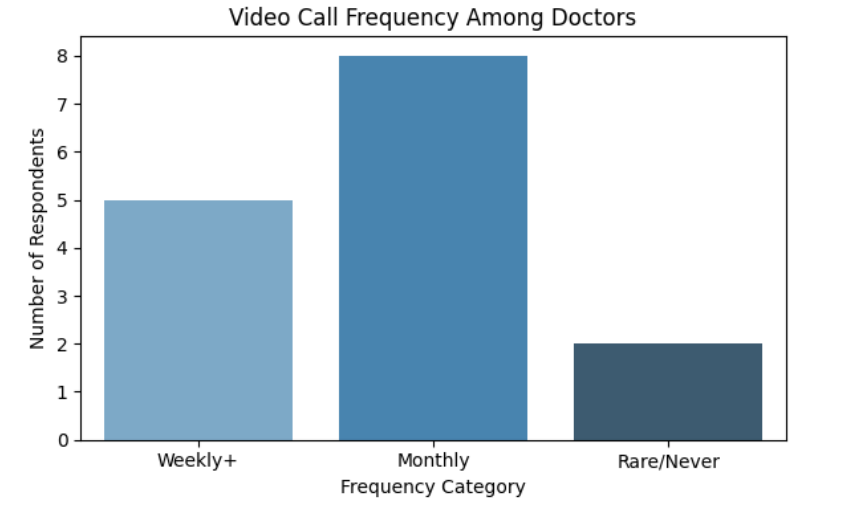
\includegraphics[width=\linewidth]{mayring_figure1.png}
\caption{Video Call Frequency}
\label{fig:mayring-video-call-frequency}
\end{figure}

Appointment scheduling remains largely manual. Most physicians rely on paper-based systems or telephone coordination, while only a small minority report using official digital scheduling systems and isolated ad hoc tools. In some urban settings, partial digital solutions such as electronic health record systems or pilot platforms exist, but these are not integrated into broader workflows. As a result, inefficiencies such as double-booking and redundant administrative work frequently occur. Figure~\ref{fig:mayring-scheduling-methods} illustrates this distribution of scheduling methods.

\begin{figure}[H]
\centering
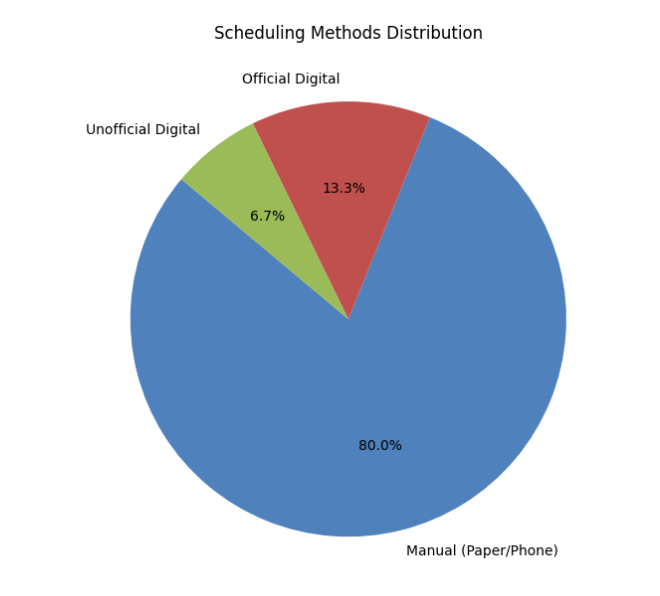
\includegraphics[width=\linewidth]{mayring_figure2.png}
\caption{Scheduling Methods Distribution}
\label{fig:mayring-scheduling-methods}
\end{figure}

Data management practices are characterized by a predominance of paper-based documentation combined with ad hoc digital storage solutions. Physicians often store patient data on personal devices, USB drives, or simple spreadsheet applications. This fragmented approach leads to significant operational risks, including frequent reports of data loss due to device failures, malware, or the absence of systematic backup procedures. Concerns regarding data security and legal uncertainty are widespread. Messaging applications are perceived as convenient, yet they are also recognized as insecure and not compliant with formal data protection standards. Many physicians further express uncertainty regarding legal responsibilities, particularly in relation to remote diagnosis, electronic prescriptions, and patient consent, which contributes to cautious behavior in remote settings. The reported prevalence of data-loss incidents is high, and legal uncertainty is nearly universal across the interview sample, as summarized in Figure~\ref{fig:mayring-data-loss-legal}.

\begin{figure}[H]
\centering
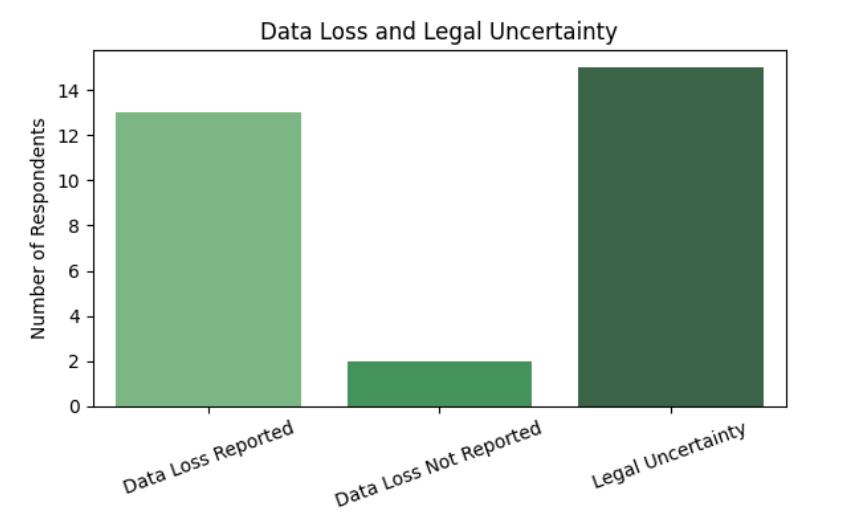
\includegraphics[width=\linewidth]{mayring_figure3.png}
\caption{Data Loss and Legal Uncertainty}
\label{fig:mayring-data-loss-legal}
\end{figure}

Another important finding relates to the impact of digital communication on work--life boundaries. Physicians report that asynchronous messaging creates expectations of constant availability, leading to increased workload outside regular working hours. This highlights the need for structured communication tools that allow better control over availability and response times. Despite these challenges, there is a clear demand for a centralized and secure telemedicine platform. Many participants emphasize the need for a government-approved solution that integrates communication, scheduling, and data management functionalities while ensuring compliance with legal and data protection requirements.

Differences between medical specialties and regional contexts are also evident. For example, cardiology shows a comparatively higher adoption of telemedicine for chronic disease management and exchange of diagnostic data, whereas surgical disciplines remain more skeptical due to the hands-on nature of their work. Urban healthcare providers tend to adopt digital tools more readily, while semi-rural and rural settings remain strongly dependent on paper-based processes.

\section{Discussion}

The findings demonstrate that telemedicine in Uzbekistan is already present in everyday clinical practice, albeit in an informal and unstructured manner. The widespread use of consumer messaging applications indicates both a strong demand for digital healthcare solutions and a lack of adequate institutional infrastructure. These observations are consistent with the broader health system challenges outlined in Chapter 1. While digital health has been identified as a strategic priority, its implementation remains uneven and constrained by infrastructural, organizational, and regulatory limitations.

From a system design perspective, the results imply several key requirements for a telemedicine platform. These include secure and compliant communication channels, integrated appointment scheduling, reliable data storage solutions, and clear mechanisms for managing legal and ethical responsibilities. In addition, user-centered features that address workload management and heterogeneous levels of digital literacy appear necessary to support adoption across diverse practice settings, in line with established adoption and implementation frameworks (Venkatesh et al., 2003; Greenhalgh et al., 2017).

\section{Conclusion}

This analysis shows that physicians in Uzbekistan are already engaging in telemedicine practices through informal digital tools, particularly for follow-up care and patient communication. However, the lack of integrated systems, combined with data security risks and legal uncertainty, limits the effectiveness and scalability of these practices. While the sample of fifteen interviews provides valuable insights across different regions and specialties, it is not statistically representative. The findings are therefore most applicable to similar healthcare contexts characterized by limited digital infrastructure and transitional regulatory environments. To enhance reliability in future work, additional validation procedures such as inter-coder agreement or participant feedback could be incorporated. Nevertheless, the results provide an empirical foundation for the development of a structured and context-appropriate telemedicine platform.


\chapter{Requirements Derived from the Qualitative Analysis}
\label{ch:requirements-derived}

\section{Introduction}

Chapter 4 synthesizes physicians' experiences with telemedicine in Uzbekistan through qualitative content analysis. The present chapter translates those findings into a structured set of system requirements and describes how the Shifa platform---comprising a patient mobile application, a doctor-oriented client with administrative capabilities, and a shared backend service---addresses them. The exposition follows a conventional engineering progression from stakeholder needs to requirements and onward to architectural realization, as developed in subsequent chapters of this document.

\section{From Practitioner Needs to System Requirements}

The interview material in Chapter 4 yields recurring themes: reliance on informal channels for communication, uneven adoption of video consultations, manual and error-prone scheduling practices, fragmented documentation and storage, concern about data protection and legal clarity, and pressure from asynchronous communication outside formal working hours. These themes are not treated as isolated anecdotes; they are abstracted into \emph{system requirements} that specify \emph{what} the platform must enable, without prescribing a single commercial product architecture.

Requirement formulation follows three principles. First, each major requirement can be traced to at least one thematic cluster in Chapter 4. Second, where implementation necessarily introduces capabilities that the interviews did not name explicitly---for example token-based API security, push notification infrastructure, or timezone-aware scheduling---these are classified as \emph{technical enablers} that support the primary clinical and organizational requirements. Third, capabilities that extend the core narrative but are not yet central to everyday practice in the sample (for example deep interoperability with national health information systems) are noted as \emph{future extensions} so that the scope of the described system remains clear without diverting the main line of argument.

\section{Functional Requirements by Domain}

Table~\ref{tab:functional-requirements-domains} summarizes functional requirement domains, their rationale in light of Chapter 4, and how the three software components collectively realize them. The division into domains follows the structure of the interview guide and the coding categories used in the qualitative analysis.

\footnotesize
\begin{longtable}{@{}>{\RaggedRight\arraybackslash}p{2.4cm}>{\RaggedRight\arraybackslash}p{4.8cm}>{\RaggedRight\arraybackslash}p{5.6cm}@{}}
\caption{Functional requirement domains derived from Chapter 4 and their realization across the Shifa platform.}\label{tab:functional-requirements-domains}\\
\toprule
\textbf{Domain} & \textbf{Requirement intent (from qualitative themes)} & \textbf{Realization in the system}\\\midrule
\endfirsthead
\toprule
\textbf{Domain} & \textbf{Requirement intent (from qualitative themes)} & \textbf{Realization in the system}\\\midrule
\endhead
\midrule
\multicolumn{3}{r@{}}{Continued on next page}\\\endfoot
\bottomrule
\endlastfoot
Identity and trust & Verified participation of doctors and patients, role-appropriate access, and session integrity. & Firebase phone authentication and JWT-backed API access; backend roles for doctor, patient, and administrator; dedicated onboarding and account flows in both clients.\\
Secure communication & Replace ad-hoc messengers with a channel that preserves clinical context and supports rich media. & Conversation-based messaging with attachments in both applications, backed by shared messaging and file APIs.\\
Video care & Support follow-up and triage-style encounters when in-person examination is limited or impractical. & Appointment-linked video sessions using a managed real-time stack (Daily.co), including waiting-room and token flows coordinated by the backend.\\
Scheduling and coordination & Reduce double-booking and manual coordination by anchoring appointments in a single source of truth. & Doctor-defined availability and calendar views; patient booking flows; appointment lifecycle and schedule APIs shared by both clients.\\
Documentation and cognitive load & Reduce documentation burden while keeping clinical judgment with the physician. & Consultation notes, AI-assisted drafting where offered, visit summaries, and structured patient-facing steps (e.g.\ signing and summary screens) aligned with backend consultation and AI endpoints.\\
Documents and continuity of information & Exchange investigations and records in a controlled way tied to the care episode. & Patient and doctor document features with upload, listing, and access mediation through the API.\\
Tasks and remote follow-up & Structure asynchronous follow-up and reminders beyond single messages. & Remote care tasks with check-in flows surfaced in both clients and task-related backend controllers.\\
Notifications and awareness & Keep participants informed about bookings, messages, and time-sensitive events. & In-app notification centers and push-oriented delivery (Firebase Cloud Messaging) with server-side notification records.\\
Administration and governance & Support operational oversight without embedding policy in application code alone. & Web-based administrative entry in the doctor build and administrator APIs for user and system management.\\
Observability and resilience (enabler) & Sustain trustworthy operation under real-world deployment constraints. & Spring Security, health endpoints, profile-based configuration, and deployment-oriented backend setup; client-side error handling and optional crash reporting on mobile.\\
\bottomrule
\end{longtable}
\normalsize

\section{Non-Functional Requirements and Quality Attributes}

Based on the identified needs, the system is expected to remain usable under variable mobile connectivity, to protect data in transit through modern transport security, and to keep latency of routine API interactions within responsive bounds for chat and booking workflows. Availability and recovery objectives depend on the chosen hosting environment; the backend is structured for containerized deployment and health checking so that operators can meet institutional targets. Accessibility and multilingual use are addressed through localized user interfaces---including multiple languages on the patient application---consistent with the cross-linguistic interview setting and the intended user base.

\section{Traceability from Qualitative Themes to Platform Capabilities}

Table~\ref{tab:traceability-themes-capabilities} links the high-level findings of Chapter 4 to the capability areas instantiated in the previous section. The mapping is intentionally coarse: it shows \emph{which} parts of the platform respond to \emph{which} empirical themes, supporting the claim that the engineering work is grounded in the qualitative evidence.

\begin{table}[H]
\centering
\caption{Qualitative themes (Chapter 4) and corresponding platform capability areas.}
\label{tab:traceability-themes-capabilities}
\begin{tabularx}{\textwidth}{@{}>{\RaggedRight\arraybackslash}X>{\RaggedRight\arraybackslash}X@{}}
\toprule
\textbf{Theme from Chapter 4} & \textbf{Capability area in the Shifa platform}\\
\midrule
Informal messaging; security and legal concern & Secure in-app messaging, authenticated access, administrative oversight\\
Video for follow-up and triage; connectivity limits & Appointment-based video, mobile-first clients, localized UI\\
Manual scheduling; coordination friction & Shared scheduling model, patient booking, doctor calendar\\
Fragmented records; fear of data loss & Documents API, consultation and visit documentation flows\\
After-hours pressure and workload & Notifications, tasks, structured asynchronous follow-up\\
Need for trustworthy institutional tooling & Backend RBAC, admin surfaces, deployment-oriented service design\\
\bottomrule
\end{tabularx}
\end{table}

\section{Phased Evolution and Future Extensions}

The platform is described in this thesis primarily in terms of its current integrated scope across patient application, doctor application, and backend. Guided by the same interview insights, further extensions---such as deeper integration with national health information infrastructure, advanced analytics dashboards for population-level monitoring, or specialized clinician-to-clinician case sharing with formal de-identification workflows---can be positioned as natural next steps once core adoption and governance processes stabilize. This subsection does not alter the normative requirements for the system as presented; it situates the described implementation within a plausible longer-term roadmap.

\section{Requirement-to-Realization Mapping}

Table~\ref{tab:requirement-realization-matrix} provides a consolidated view suitable for review: each row states a requirement derived from or motivated by Chapter 4, elaborates it briefly, and indicates which major software component contributes to satisfying it. A checkmark denotes primary responsibility; ``support'' denotes a contributing or enabling role (for example the backend for almost all cross-client features).

\footnotesize
\begin{longtable}{@{}>{\RaggedRight\arraybackslash}p{2.6cm}>{\RaggedRight\arraybackslash}p{4.2cm}>{\RaggedRight\arraybackslash}p{1.7cm}>{\RaggedRight\arraybackslash}p{1.7cm}>{\RaggedRight\arraybackslash}p{1.7cm}@{}}
\caption{Requirements and their realization across doctor client, patient client, and backend.}\label{tab:requirement-realization-matrix}\\
\toprule
\textbf{Requirement} & \textbf{Description} & \textbf{Doctor} & \textbf{Patient} & \textbf{Backend}\\
\midrule
\endfirsthead
\toprule
\textbf{Requirement} & \textbf{Description} & \textbf{Doctor} & \textbf{Patient} & \textbf{Backend}\\
\midrule
\endhead
\midrule
\multicolumn{5}{r@{}}{Continued on next page}\\\endfoot
\bottomrule
\endlastfoot
Authenticated access & Users prove identity and receive role-appropriate API access. & \checkmark & \checkmark & \checkmark\\
Role separation & Clinical, patient, and administrative actions are separated by authorization. & \checkmark & \checkmark & \checkmark\\
Doctor onboarding & New physicians can enter the platform through controlled onboarding paths. & \checkmark & --- & \checkmark\\
Patient registration and profile & Patients establish accounts and maintain profile data for care coordination. & --- & \checkmark & \checkmark\\
Secure messaging & Contextual chat replaces informal messengers for care-related dialogue. & \checkmark & \checkmark & \checkmark\\
Media exchange & Images and files support clinical communication (e.g.\ investigations). & \checkmark & \checkmark & \checkmark\\
Video visits & Remote encounters support follow-up and triage within appointment structure. & \checkmark & \checkmark & \checkmark\\
Scheduling integrity & Appointments are created and updated against shared server state. & \checkmark & \checkmark & \checkmark\\
Doctor availability & Physicians define when they can be booked. & \checkmark & --- & \checkmark\\
Clinical documentation & Notes and summaries capture encounter content for continuity of care. & \checkmark & \textit{support} & \checkmark\\
AI-assisted drafting & Optional assistance reduces documentation burden under physician control. & \checkmark & \textit{support} & \checkmark\\
Patient visit workflow & Patients complete steps tied to visits (e.g.\ confirmation, summary). & --- & \checkmark & \checkmark\\
Document repository & Structured storage and retrieval of patient-associated files. & \checkmark & \checkmark & \checkmark\\
Remote tasks & Structured follow-up complements unstructured messages. & \checkmark & \checkmark & \checkmark\\
Notifications & Users are alerted to relevant events. & \checkmark & \checkmark & \checkmark\\
Administration & Operational management without redeploying application code. & \checkmark & --- & \checkmark\\
Public discovery & Patients can find and select doctors for booking. & --- & \checkmark & \checkmark\\
Deployment and health & Service can be operated with monitoring and controlled configuration. & --- & --- & \checkmark\\
\bottomrule
\end{longtable}
\normalsize

\section{Scope Statement}

To address the requirements identified in Chapter 4 within a manageable engineering scope, the thesis describes an integrated telemedicine platform centered on authenticated communication, appointment-based video, shared scheduling, documentation, documents, tasks, and notifications across two client applications and one backend. Extensions that would primarily serve national-scale interoperability or specialized secondary-use research workflows remain outside the core requirement set for this document, while remaining compatible with the architecture described in the following chapters.

\chapter{User Interface and User Experience (Patient and Doctor Apps)}
\label{ch:ui-ux}

\section{Overview}

This chapter documents the user interface (UI) and user experience (UX) of the patient and doctor applications. The screenshots are grouped by application and by primary workflow intent (onboarding, scheduling, documentation, and video consultation).

To keep the layout consistent and readable, screenshots are displayed in a two-up grid (two images per figure row). Each figure row contains a shared caption describing the two screens shown.

\section{Wireframing to UI Solution}

The interface concepts were developed through iterative wireframing before producing the final high-fidelity UI screens. To illustrate this process transparently, the following figures include the complete patient-app wireframe set. The doctor-app UI was developed through the same workflow-first wireframing approach; representative final screens are shown in the next section.

\newcommand{\TwoUpWireP}[4]{%
  \begin{figure}[H]
  \centering
  \setlength{\fboxsep}{0pt}
  \begin{minipage}{0.48\linewidth}
    \centering
    \fbox{\includegraphics[width=\linewidth,height=0.26\textheight,keepaspectratio]{#1}}
  \end{minipage}\hfill
  \begin{minipage}{0.48\linewidth}
    \centering
    \fbox{\includegraphics[width=\linewidth,height=0.26\textheight,keepaspectratio]{#2}}
  \end{minipage}
  \caption{Patient wireframes: #3}
  \label{#4}
  \end{figure}
}

\TwoUpWireP{ux_wireframes/patient/wireframe_get_started_p.png}{ux_wireframes/patient/wireframe_sign_in_p.png}{Get started and sign-in entry}{fig:wf_patient_entry}
\TwoUpWireP{ux_wireframes/patient/wireframe_create_account_p.png}{ux_wireframes/patient/wireframe_create_p.png}{Create account and registration (step 1)}{fig:wf_patient_create_1}
\TwoUpWireP{ux_wireframes/patient/wireframe_create_p_1.png}{ux_wireframes/patient/wireframe_create_p_2.png}{Registration flow (steps 2--3)}{fig:wf_patient_create_2}
\TwoUpWireP{ux_wireframes/patient/wireframe_create_p_3.png}{ux_wireframes/patient/wireframe_account_success_p.png}{Registration (final step) and success}{fig:wf_patient_create_3}
\TwoUpWireP{ux_wireframes/patient/wireframe_home_p.png}{ux_wireframes/patient/wireframe_bookings_p.png}{Home and bookings overview}{fig:wf_patient_home_bookings}
\TwoUpWireP{ux_wireframes/patient/wireframe_appointment_details_p.png}{ux_wireframes/patient/wireframe_documents_p.png}{Appointment details and documents list}{fig:wf_patient_appt_docs}
\TwoUpWireP{ux_wireframes/patient/wireframe_documents_p_1.png}{ux_wireframes/patient/wireframe_profile_p.png}{Document detail and profile}{fig:wf_patient_docs_profile}
\TwoUpWireP{ux_wireframes/patient/wireframe_profile_image_p.png}{ux_wireframes/patient/wireframe_account_info_p.png}{Profile image and account information}{fig:wf_patient_profile_account}

\section{Doctor App UI Screens}

The following sections present the realized UI screens of both applications. While the wireframes capture structure and workflow intent, the final screens refine visual hierarchy, typography, and interaction affordances for practical daily use.

\newcommand{\TwoUpDoctor}[5]{%
  \begin{figure}[H]
  \centering
  \setlength{\fboxsep}{0pt}
  \begin{minipage}{0.48\linewidth}
    \centering
    \fbox{\includegraphics[width=\linewidth,height=0.26\textheight,keepaspectratio]{#1}}
  \end{minipage}\hfill
  \begin{minipage}{0.48\linewidth}
    \centering
    \fbox{\includegraphics[width=\linewidth,height=0.26\textheight,keepaspectratio]{#2}}
  \end{minipage}
  \caption{Doctor app screens: #5}
  \end{figure}
}

\TwoUpDoctor{ui_screens/doctor/doctor_loading_1.jpg}{ui_screens/doctor/doctor_loading_2.jpg}{Loading screen (variant 1)}{Loading screen (variant 2)}{Loading and initialization}
\TwoUpDoctor{ui_screens/doctor/doctor_create_account.jpg}{ui_screens/doctor/doctor_create_account_confirm.jpg}{Create account}{Account creation confirmation}{Doctor onboarding}
\TwoUpDoctor{ui_screens/doctor/doctor_account_information.jpg}{ui_screens/doctor/doctor_profile_image.jpg}{Account information}{Profile image}{Account setup}
\TwoUpDoctor{ui_screens/doctor/doctor_profile.jpg}{ui_screens/doctor/doctor_home.jpg}{Doctor profile}{Doctor home dashboard}{Profile and daily work}

\TwoUpDoctor{ui_screens/doctor/doctor_calendar_setup_intro.jpg}{ui_screens/doctor/doctor_calendar_setup_1.jpg}{Calendar setup introduction}{Availability input}{Calendar setup}
\TwoUpDoctor{ui_screens/doctor/doctor_calendar_setup_2.jpg}{ui_screens/doctor/doctor_calendar_setup_3.jpg}{Slot configuration}{Exceptions/controls}{Scheduling rules}
\TwoUpDoctor{ui_screens/doctor/doctor_calendar_setup_4.jpg}{ui_screens/doctor/doctor_calendar_setup_5.jpg}{Review and persistence}{Final confirmation}{Calendar finalization}

\TwoUpDoctor{ui_screens/doctor/doctor_patients.jpg}{ui_screens/doctor/doctor_attach_patient.jpg}{Patients list}{Attach patient context}{Patient context workflow}
\TwoUpDoctor{ui_screens/doctor/doctor_schedule_edit.jpg}{ui_screens/doctor/doctor_documents.jpg}{Schedule edit}{Document management}{Availability updates and records}

\TwoUpDoctor{ui_screens/doctor/doctor_start_appointment.jpg}{ui_screens/doctor/doctor_start_appointment_confirm.jpg}{Start appointment}{Start appointment confirmation}{Encounter initiation}

% Odd number of screenshots: the remaining screen is shown as a single figure.
\begin{figure}[H]
\centering
\setlength{\fboxsep}{0pt}
\fbox{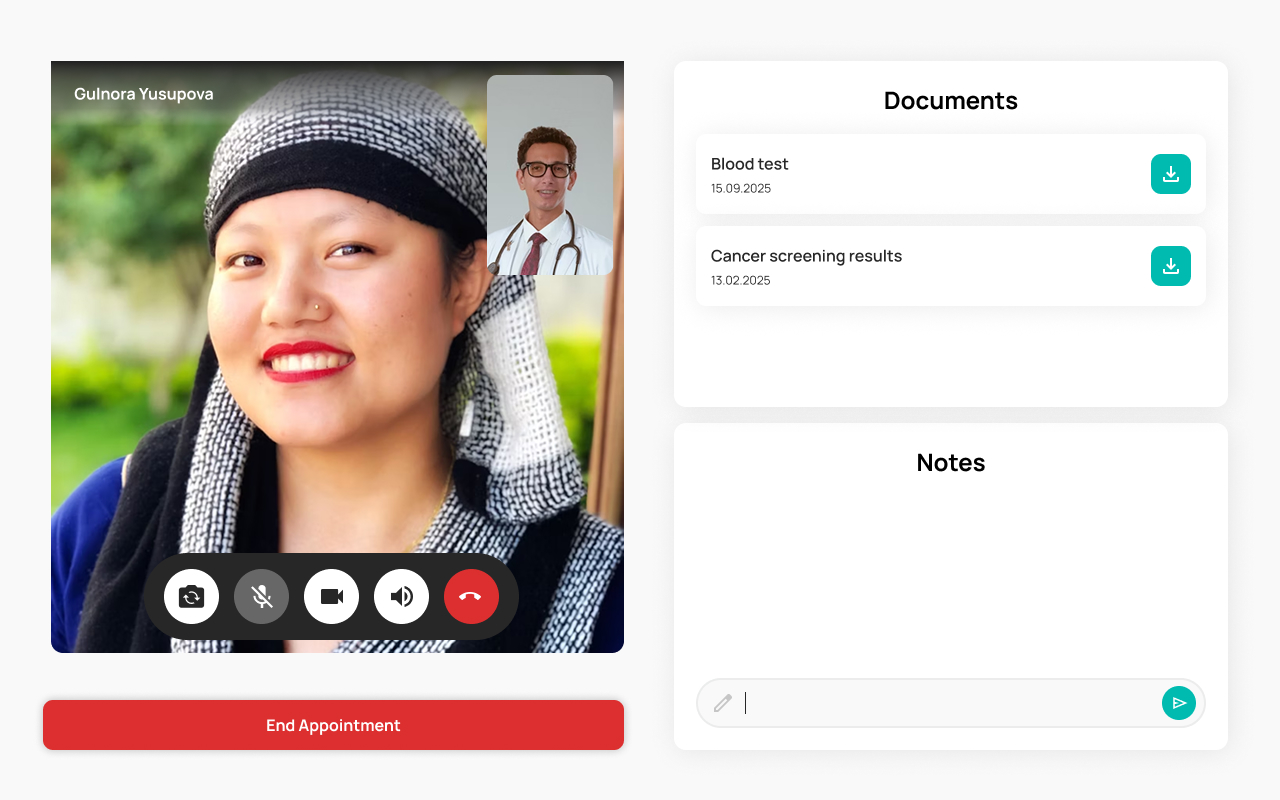
\includegraphics[width=0.72\linewidth,height=0.26\textheight,keepaspectratio]{ui_screens/doctor/doctor_join_video.jpg}}
\caption{Doctor app: video consultation join}
\end{figure}

\section{Patient App UI Screens}

\newcommand{\TwoUpPatient}[5]{%
  \begin{figure}[H]
  \centering
  \setlength{\fboxsep}{0pt}
  \begin{minipage}{0.48\linewidth}
    \centering
    \fbox{\includegraphics[width=\linewidth,height=0.26\textheight,keepaspectratio]{#1}}
  \end{minipage}\hfill
  \begin{minipage}{0.48\linewidth}
    \centering
    \fbox{\includegraphics[width=\linewidth,height=0.26\textheight,keepaspectratio]{#2}}
  \end{minipage}
  \caption{Patient app screens: #5}
  \end{figure}
}

\TwoUpPatient{ui_screens/patient/patient_loading.png}{ui_screens/patient/patient_loading_2.png}{Loading screen (variant 1)}{Loading screen (variant 2)}{Startup and readiness}
\TwoUpPatient{ui_screens/patient/patient_get_started.png}{ui_screens/patient/patient_create_account.png}{Get started}{Create account}{Onboarding}

\TwoUpPatient{ui_screens/patient/patient_create_flow_1.png}{ui_screens/patient/patient_create_flow_2.png}{Create flow step 1}{Create flow step 2}{Account creation flow}
\TwoUpPatient{ui_screens/patient/patient_create_flow_3.png}{ui_screens/patient/patient_create_flow_4.png}{Create flow step 3}{Create flow step 4}{Account creation flow (continued)}
\TwoUpPatient{ui_screens/patient/patient_create_flow_5.png}{ui_screens/patient/patient_home.png}{Create flow step 5}{Home}{Account confirmation and home}

\TwoUpPatient{ui_screens/patient/patient_bookings.png}{ui_screens/patient/patient_doctors.png}{Bookings}{Doctors list}{Selecting a provider}
\TwoUpPatient{ui_screens/patient/patient_doctors_detail.png}{ui_screens/patient/patient_documents.png}{Doctor details}{Documents list}{Provider overview and records}
\TwoUpPatient{ui_screens/patient/patient_documents_detail.png}{ui_screens/patient/patient_profile.png}{Document detail}{Profile overview}{Viewing documents and profile}

\TwoUpPatient{ui_screens/patient/patient_profile_menu.png}{ui_screens/patient/patient_profile_image.png}{Profile menu}{Profile image}{Profile settings}
\TwoUpPatient{ui_screens/patient/patient_account_info.png}{ui_screens/patient/patient_appointment_upcoming.png}{Account info}{Upcoming appointment}{Appointments overview}
\TwoUpPatient{ui_screens/patient/patient_appointment_upcoming_2.png}{ui_screens/patient/patient_appointment_past.png}{Upcoming details (variant)}{Past appointment}{Appointment details}
\TwoUpPatient{ui_screens/patient/patient_waiting_room.png}{ui_screens/patient/patient_video_call.png}{Waiting room}{Video consultation}{Video encounter}

\section{Cross-Cutting UX Considerations}

Across both applications, the UX is organized around clinical intent units: (1) confirm identity and session integrity, (2) establish appointment context, (3) communicate and exchange supporting information, and (4) preserve continuity of care through documents and encounter summaries.

The doctor application emphasizes availability configuration and encounter initiation as primary first-class actions. The patient application emphasizes booking discoverability and appointment awareness through lists and detail screens. Both clients support asynchronous workflow continuity via tasks and notifications.

The present chapter therefore focuses on design and implemented interaction structure, while the evaluation design and methodological framing for assessing usability, acceptability, and perceived impact are discussed in later chapters as part of the ongoing prototype evaluation.



\clearpage

\chapter{System Architecture Overview}
\label{ch:system-architecture}

\section{System context}

Following the empirical findings in Chapter~4 and the requirements synthesis in Chapter~5, this thesis implements a concrete three-tier telemedicine prototype with two client applications and one central backend service. The architecture is intentionally scoped to the study constraints: requirements were derived primarily from 15 physician interviews and then reconciled against what could be delivered as a working system within the thesis timeline. Patients use the mobile client for onboarding, appointments, messaging, documents, and video participation, while doctors and administrators use the web client for schedule control, patient workflows, communication, and operational oversight. This framing emphasizes executable integration rather than a purely conceptual platform model.

From a technical perspective, the system consists of a Flutter-based patient application, a Flutter Web doctor/admin application hosted on Firebase Hosting, and a Kotlin/Spring Boot backend service that exposes REST APIs and persists data in PostgreSQL. The backend integrates with Firebase for phone authentication (OTP) and push notifications and with Daily.co for video rooms and media transport via the \texttt{daily\_flutter} SDK. The backend and database are deployed on Railway (or an equivalent PaaS), while the mobile and web clients are distributed via app stores and web hosting.

The following subsection makes this alignment explicit with respect to the research questions (Chapter~1.2).

\subsection{Architectural Alignment with Research Questions}

The architecture described in this chapter is not merely an implementation artefact detached from the empirical programme of the thesis. It operationalises the chain from problem analysis to design: qualitative findings on everyday practice in Uzbekistan (see Chapter~4) inform a structured requirement baseline (see Chapter~5), which in turn constrains how the prototype is partitioned into clients, services, and integrations. Stating this alignment explicitly reduces the risk that technical description reads as generic platform marketing: each major container and integration choice should be traceable back to a documented need or requirement domain, while remaining honest about prototype scope and unresolved risks treated elsewhere in the document.

\textbf{Alignment with the physician-centred research question (RQ2).} Chapter~4 documents recurrent service-delivery inefficiencies among interviewed physicians: reliance on informal messaging applications and telephone for patient contact, manual appointment coordination prone to error and duplication, fragmented digital documentation and ad hoc storage associated with data loss, legal uncertainty around remote practice, and pressure to remain available outside formal working hours. The implemented architecture responds to these themes by concentrating coordination in a single backend that maintains shared appointment and scheduling state, so that booking and calendar views for doctors and patients refer to the same persisted records rather than parallel informal channels. In-app messaging and notification flows routed through authenticated APIs offer a structured substitute for consumer messaging tools, preserving thread context tied to care relationships rather than dispersed chat logs. Task and follow-up constructs, together with notification delivery via Firebase Cloud Messaging, support asynchronous continuity of care and can help bound expectations compared with unbounded messaging expectations. The separation of the doctor-facing web client from the patient mobile client, with an additional administrative entry on the web stack, mirrors role differences in workflow control: clinical and operational work is grouped where physicians and administrators actually perform it, while patients encounter a journey-oriented mobile surface. This mapping is intentional: the goal is to reduce the coordination failures and cognitive overhead described in Chapter~4 without pretending that software alone resolves legal or organisational ambiguity.

\textbf{Alignment with requirements and design decisions (RQ3).} Chapter~5 organises the derived platform needs into domains that include identity and trust, secure communication, video-mediated care, scheduling and coordination, documentation and cognitive load, documents, tasks and follow-up, notifications, administrative governance, and observability or resilience. The two-client split follows directly from differing roles and information needs: patients require discovery, booking, and self-service access to their own data; doctors require schedule management, patient lists, messaging, and operational tools. The Spring Boot backend functions as an orchestration kernel: it exposes REST contracts consumed by both clients, enforces role-based access after Firebase-supported OTP and backend-issued JWT authentication, and persists authoritative state in PostgreSQL rather than leaving clinical coordination to disconnected spreadsheets or messaging threads. Video encounters are delegated to Daily.co with tokens issued by the backend, which matches the interview emphasis on follow-up and triage-style remote contact while acknowledging limits of remote examination. Push notifications via Firebase support timely prompts within the notification domain. Optional AI-assisted features, where present in the broader system context, remain bounded integrations rather than the core trust anchor; the primary trust mechanism in the prototype remains authenticated access to shared records and controlled workflows. Together, these decisions instantiate the requirement domains as implementable services rather than as abstract wish lists.

\textbf{Alignment with evaluation and patient-centred inquiry (RQ4; RQ1).} The fourth research question concerns user response to the prototype and feedback on access and efficiency implications; evaluation is ongoing and will be reported in the empirical chapters of the thesis rather than asserted here. Architecturally, the prototype is nevertheless shaped to make such evaluation feasible: end-to-end executable paths exist from authentication through booking, messaging, document-related workflows, and video participation, so that usability, acceptability, and perceived impact can be observed on realistic task sequences rather than on isolated screens. The backend's retention of appointment lifecycle state, message and notification events, and audit-relevant server-side logs provides a basis for correlating subjective reports with objective traces where ethically and methodologically appropriate, without claiming that full instrumentation or formal service-level measurement is already in place. The separation of patient journey surfaces from doctor workflow surfaces also supports differentiated evaluation instruments and sampling strategies. The first research question, on patient-perceived access barriers and the role of digital tools, is only partly addressed in the present thesis through complementary patient perspective input (see Chapter~4 methodology); the mobile client and booking architecture anticipate common access mechanisms (remote appointment booking, messaging, video), but the architecture chapter does not substitute for dedicated patient evidence where that evidence is still forthcoming.

\textbf{Limits of what the architecture claims.} This prototype is not presented as nationally scalable infrastructure, as fully compliant with all data-protection regimes, or as interoperable with legacy institutional systems without further integration work. Deployment choices prioritise feasibility and reproducibility over geo-redundancy and formal service-level operations, consistent with Section~7.4 and with the limitations chapter. Known security and testing gaps documented later in the thesis remain part of the honest boundary of the artefact. The alignment argument here is therefore modest: the architecture is a traceable response to empirically grounded requirements within thesis constraints, not a certificate of production readiness.

\section{System context diagram (C4 Level 1)}

The overall placement of actors and technical systems is illustrated in the system context diagram (C4 Level 1) reproduced in Figure~\ref{fig:system-context}. This figure shows patients and doctors as external actors using the two Flutter-based clients, which in turn communicate exclusively with the central backend service. The backend delegates authentication and notification tasks to Firebase, outsources media transport for video encounters to Daily.co, and persists all core state to PostgreSQL.

\ShifaFigSystemContext

\section{Container architecture (C4 Level 2)}

At container level, three main software containers cooperate: the patient app (Flutter mobile), the doctor/admin app (Flutter Web SPA), and the backend (Spring Boot monolith). The patient app encapsulates all patient-facing workflows, including onboarding, bookings, documents, messaging, and video participation. The doctor/admin app encapsulates doctor- and administrator-facing workflows such as dashboards, calendar views, patient lists, messaging, tasks, analytics, and configuration tools. The backend encapsulates persistence, domain logic, and integration with PostgreSQL, Firebase, and Daily.co, and exposes REST APIs that decouple client development from internal implementation choices.

Conceptually, authentication proceeds by using Firebase phone OTP where applicable, after which the backend issues JWTs that are attached to subsequent REST requests. Appointment and schedule management proceeds by having the patient app initiate bookings, the backend create and manage appointment state, and the doctor app render calendar and appointment details from API responses. Messaging and document exchange are handled by both clients sending and retrieving messages and document metadata via REST, with the backend storing structured records in PostgreSQL and files in configured storage. Video consultations are orchestrated by the clients requesting join tokens from the backend, which integrates with Daily.co; clients then join video rooms using the \texttt{daily\_flutter} SDK. Together, these flows implement the requirement clusters E1--E7 and E9--E12 from Chapter~5.

\section{Deployment viewpoint}

The deployment topology places the backend and PostgreSQL database on Railway (or an equivalent PaaS), using health checks and environment-specific configuration profiles. In this project, deployment decisions prioritize implementation feasibility and reproducibility over high-assurance infrastructure patterns such as multi-region failover. The patient app is distributed via mobile channels and connects over HTTPS to backend and Firebase services; the doctor/admin app is deployed as a Flutter Web SPA on Firebase Hosting with separate hostnames for doctor and admin entry. This is therefore an operational prototype baseline, not a claim of national-scale production readiness. The deployment structure and external integrations are illustrated further in Section~\ref{ch:backend-implementation}.

Taken together, this deployment posture should be read as prototype-grade and oriented toward supporting user-centred evaluation, rather than as evidence that the system already satisfies production-ready operational standards.

\chapter{Backend Implementation}
\label{ch:backend-implementation}

\section{System Architecture Overview}

At backend level, the Shifa platform operates as the integration and coordination point between two Flutter-based clients and several external services. Patients and doctors are the primary actors: patients interact with the patient mobile application to perform the workflows analysed in Chapters~4--6, whereas doctors (and administrators) interact with the web-based doctor application to manage clinical work. Both clients communicate exclusively with the backend via REST over HTTPS. The backend, in turn, relies on PostgreSQL for persistence, Firebase for phone-based authentication and notifications, and Daily.co for media transport in video consultations.

The system context for the backend is thus identical in structure to the global platform context shown in Chapter~\ref{ch:system-architecture}. For convenience, Figure~\ref{fig:backend-system-context} reproduces the same diagram rendered at backend chapter scope.

\begin{figure}[H]
\centering
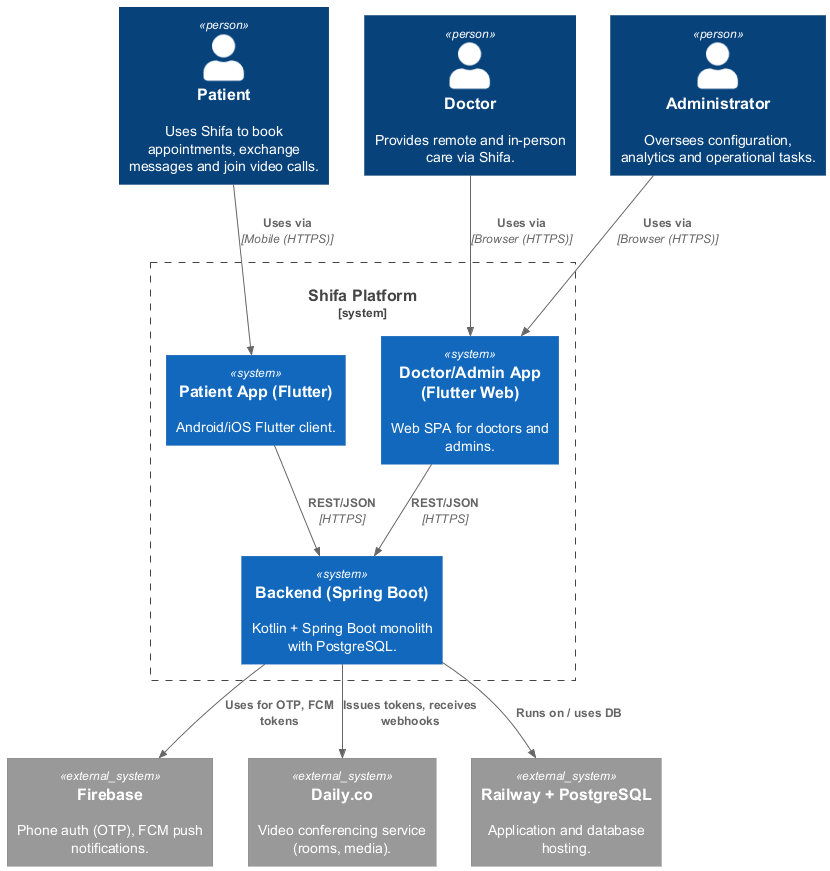
\includegraphics[width=\linewidth]{diagrams/fig_7_1_system_context.png}
\caption{Backend-centred system context diagram (C4 Level 1).}
\label{fig:backend-system-context}
\end{figure}

At container level, the same three platform containers (patient app, doctor app, backend API) appear together with PostgreSQL, Firebase, and Daily.co; Figure~\ref{fig:backend-container-arch} shows this view for the backend in isolation.

\begin{figure}[H]
\centering
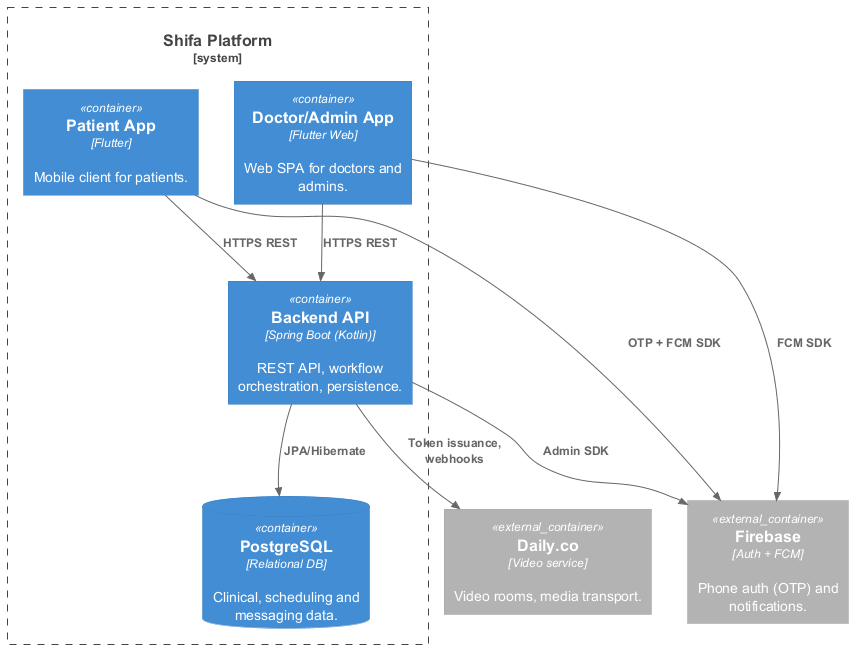
\includegraphics[width=\linewidth]{diagrams/fig_7_2_containers.png}
\caption{Backend-centred container architecture (C4 Level 2).}
\label{fig:backend-container-arch}
\end{figure}

\section{Role in the overall solution}

Following the requirement synthesis in Chapter~5 and the workflow evidence in Chapter~4, the backend acts as the coordination layer between both clients. It is implemented as a Spring Boot service in Kotlin, with PostgreSQL persistence and Flyway-based schema evolution. Analytically, the backend fulfills three roles: (1) identity and authorization control, (2) workflow orchestration for appointments, messaging, documents, and tasks, and (3) stable API contracts for mobile and web clients.

\section{Architecture and layering}

The internal structure follows a conventional layered organization: web controllers as API adapters, services for business logic, repositories for database access, domain entities for persistence models, and cross-cutting security/configuration modules. This architecture is technically simple enough for maintainability, while still supporting the complexity of the integrated telemedicine workflow.

\ShifaFigBackendLayers
\ShifaFigJwtFlow

\section{Technology baseline}

The backend is implemented with Spring Boot~3.3.x and Kotlin~2.0.x on Java~21. Core modules include Spring Web, Validation, Actuator, Data JPA, Security, Flyway, and PostgreSQL integration. Additional technical modules include JWT processing, caching, optional rate-limiting support, and integrations for Firebase and PDF processing. This stack supports the trust and continuity requirements discussed in Chapter~5 while remaining compatible with iterative domain evolution.

\section{Data model and persistence strategy}

The persistence model is centered on users and roles, doctor and patient profiles, appointments, messages, notifications, documents, and remote-care tasks. These entities support the thematic needs identified in Chapter~4: continuous communication, appointment reliability, and continuity of clinical records. Database changes are versioned through Flyway migrations, which allows traceable schema evolution during iterative development.

The domain package contains a broad entity set, including appointment, consultation note, conversation, document access, task, notification, and schedule rule entities. This breadth indicates that the implemented backend already operates as an integrated clinical workflow kernel rather than as a single-feature prototype.

The central ownership and relationship structure is summarised in Figure~\ref{fig:backend-er}. It highlights that users are associated with roles and profiles, that appointments always link one doctor and one patient profile, that messages are anchored in conversations and sent by users, and that documents and tasks are patient-centric but involve doctors as assigners or consumers.

\begin{figure}[H]
\centering
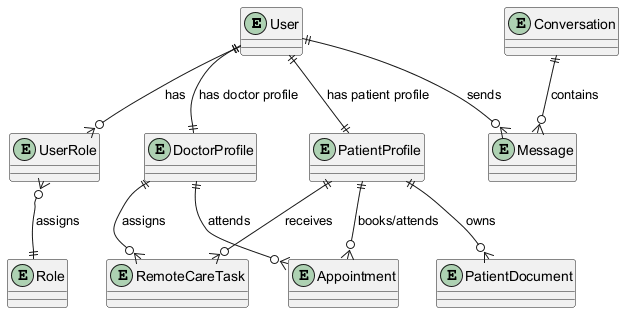
\includegraphics[width=0.9\linewidth]{diagrams/fig_7_3_er.png}
\caption{Backend data relationships (ER-style sketch).}
\label{fig:backend-er}
\end{figure}

From the perspective of the qualitative findings, this persistence model is not only a technical schema but a response to recurring practice-level problems in Uzbekistan (see Chapter~4): fragmented documentation, manual coordination, and data-loss exposure in loosely coupled tools. By maintaining appointments, conversations/messages, documents, tasks, and notifications in a shared PostgreSQL model with Flyway-governed evolution, the backend creates a single continuity layer across patient and doctor workflows. This directly supports the requirement traceability logic in Chapter~5 and contributes to RQ2 and RQ3 in Chapter~1.2 by translating physician-reported inefficiencies into auditable data structures and coordination state.

\section{API surface and core domains}
\label{ch:api}

At the API level, the backend exposes endpoints for authentication, doctor discovery, patient and doctor self-service profiles, appointment booking and lifecycle management, scheduling, messaging and attachments, documents and access requests, video tokens/webhooks, notifications, tasks, and AI-assisted clinical functions.

The endpoint design is resource-oriented and grouped by domain prefixes (for example \path{/api/auth}, \path{/api/patients}, \path{/api/appointments}, \path{/api/messages}, \path{/api/video}, and \path{/api/admin}). This domain grouping supports clearer client integration and helps maintain conceptual separation between patient-facing, doctor-facing, and administrative operations.

\textbf{Implementation status.} Implemented in the current prototype: controller-level endpoint structure and base-path grouping as documented in Table~\ref{tab:api-prefixes}. Partially implemented / currently limited: the thesis provides auditable endpoint groups but not a machine-readable contract with full operation-level schemas. Planned improvement (future work): export OpenAPI definitions from controllers and/or enforce contract tests in CI to keep API behaviour verifiable during iteration.

\footnotesize
\begin{longtable}{@{}>{\RaggedRight\arraybackslash}p{5.2cm}>{\RaggedRight\arraybackslash}p{6.8cm}@{}}
\caption{REST controller base paths (backend).} \label{tab:api-prefixes} \\
\toprule
\textbf{Controller} & \textbf{Base path} \\
\midrule
\endfirsthead
\multicolumn{2}{c}{\tablename\ \thetable{} --- continued} \\
\toprule
\textbf{Controller} & \textbf{Base path} \\
\midrule
\endhead
\midrule
\multicolumn{2}{r}{\emph{Continued on next page}} \\
\endfoot
\bottomrule
\endlastfoot
\texttt{AdminController} & \path{/api/admin} \\
\texttt{AppointmentController} & \path{/api/appointments} \\
\texttt{AuthController} & \path{/api/auth} \\
\texttt{BookingController} & \path{/api/schedule/book} \\
\texttt{CalendarController} & \path{/api/calendar} \\
\texttt{ConsultationController} & \path{/api/consultations} \\
\texttt{DoctorController} & \path{/api/doctors/me} \\
\texttt{MessageController} & \path{/api/messages} \\
\texttt{NotificationController} & \path{/api/notifications} \\
\texttt{PatientAppointmentController} & \path{/api/patients/me/appointments} \\
\texttt{PatientController} & \path{/api/patients/me} \\
\texttt{PatientDocumentController} & \path{/api/patients} \\
\texttt{PatientMessageController} & \path{/api/patients/me/messages} \\
\texttt{PatientScheduleController} & \path{/api/patients/me/schedule} \\
\texttt{RemoteCareTaskController} & \path{/api/tasks} \\
\texttt{ScheduleController} & \path{/api/schedule} \\
\texttt{VideoController} & \path{/api/video} \\
\end{longtable}
\normalsize

\subsection{Illustrative API Endpoint Example}

To complement Table~\ref{tab:api-prefixes}, this subsection documents one representative method-level endpoint used in the implemented prototype. The example is intentionally illustrative rather than exhaustive: it demonstrates how route grouping, authentication, and workflow purpose are aligned, but it does not constitute a full API contract. Accordingly, this example supports readability of the architectural argument and does not replace a complete OpenAPI-style specification.

\begin{table}[H]
\centering
\caption{Illustrative endpoint documentation for patient appointment booking.}
\label{tab:illustrative-endpoint}
\begin{tabularx}{\textwidth}{@{}>{\RaggedRight\arraybackslash}p{4.4cm}>{\RaggedRight\arraybackslash}p{2.1cm}>{\RaggedRight\arraybackslash}p{4.2cm}>{\RaggedRight\arraybackslash}X@{}}
\toprule
\textbf{Endpoint} & \textbf{HTTP Verb} & \textbf{Authentication / Authorization} & \textbf{Purpose in the system} \\
\midrule
\codepath{/api/patients/me/}\\\codepath{appointments} & \texttt{POST} & JWT bearer token required; role-scoped access for authenticated patient context via RBAC and ownership checks. & Creates a patient appointment request in shared backend state, enabling coordinated scheduling between patient and doctor workflows. \\
\bottomrule
\end{tabularx}
\end{table}

\noindent\textbf{Illustrative request body (conceptual):}
\begin{verbatim}
{
  "doctorId": 42,
  "startTimeUtc": "2026-04-10T09:30:00Z",
  "visitType": "VIDEO",
  "notes": "Follow-up consultation"
}
\end{verbatim}

\noindent\textbf{Illustrative response body (conceptual):}
\begin{verbatim}
{
  "appointmentId": 981,
  "status": "BOOKED",
  "doctorId": 42,
  "patientId": 315,
  "startTimeUtc": "2026-04-10T09:30:00Z"
}
\end{verbatim}

For a thesis-stage prototype, one concrete endpoint illustration is sufficient to demonstrate method-level API semantics without overstating contract maturity. This example links Chapter~1 objectives to executable backend behaviour, preserves traceability to the scheduling and coordination requirement domains in Chapter~5, and supports evaluation readiness for RQ4 by making the booking workflow inspectable in end-to-end tests. Full contract formalization remains planned future work.

\section{Backend Component Architecture}

The component structure can be summarised as three cooperating layers. Controllers under \path{com.shifa.web} translate HTTP requests into typed Kotlin calls. Services under \path{com.shifa.service} implement workflow logic such as appointment lifecycle transitions and document access checks, while repositories under \path{com.shifa.repo} encapsulate JPA-based persistence against PostgreSQL. This organisation allows each layer to evolve independently; for example, HTTP contracts can change without touching data access code, and persistence optimisations can occur without altering business rules. Figure~\ref{fig:backend-components} visualises this layering.

\begin{figure}[H]
\centering
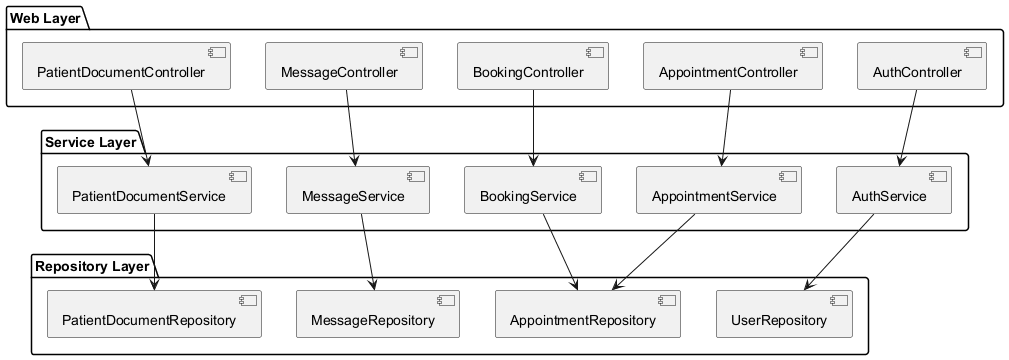
\includegraphics[width=0.9\linewidth]{diagrams/fig_7_4_components.png}
\caption{Backend component layering (controllers, services, repositories).}
\label{fig:backend-components}
\end{figure}

\section{Security and reliability}

Security is based on JWT-authenticated requests with role-aware authorization rules. The implemented role model includes doctor, patient, and administrator roles. Operationally, the service includes profile-based configuration (development, QA, production), health endpoints for deployment monitoring, and optional request-rate controls via Bucket4j.

For resilience, the backend is deployment-ready for containerized environments, with environment-driven configuration and production profile hardening (for example validated schema mode and reduced debug verbosity). This design aligns with Chapter~5 requirements on trust, stability, and controlled access.

\ShifaFigSecurityRisk
\ShifaFigDeployment

\section{Security architecture}

In addition to the general considerations above, the backend implements a concrete security architecture based on JWT lifecycle management and role-based access control. After successful authentication, the backend issues a JWT containing the user identifier and role claims (\texttt{DOCTOR}, \texttt{PATIENT}, or \texttt{ADMIN}). Clients attach this token via the \texttt{Authorization: Bearer} header on subsequent requests, and Spring Security filters validate the token and derive the security context for controller methods.

\textbf{Implementation status.} Implemented in the current prototype: OTP-assisted login flow with backend-issued JWTs, role-claim enforcement in Spring Security, and authenticated access checks across most API domains. Partially implemented / currently limited: JWT handling does not yet provide robust token revocation/rotation controls at production depth, and there is no systematic CI-backed regression suite for security routes. Planned improvement (future work): strengthen token lifecycle controls and add automated security tests (including 401/403 boundary checks) to make authentication and authorization behaviour continuously auditable.

The most relevant vulnerabilities observed in the current code are, first, the static exposure of patient documents via the \path{/patientdocuments/**} URL pattern combined with a permissive security rule, and second, the lack of systematic regression tests for security-relevant routes. This means document access control is not yet fully compliant with the confidentiality target described in Chapter~5. The first vulnerability is therefore treated as unresolved and high severity in the current prototype; mitigation is planned by routing all document access through authenticated controller methods that enforce ownership checks and, where appropriate, issue short-lived signed URLs for temporary access. The second vulnerability is planned to be mitigated by introducing dedicated security tests that verify 401/403 responses across representative endpoints and integrating these tests into CI.

The high-level authentication and authorisation flow is visualised in Figure~\ref{fig:backend-auth-arch}, which emphasises the interaction between client, backend, and Spring Security filters.

\begin{figure}[H]
\centering
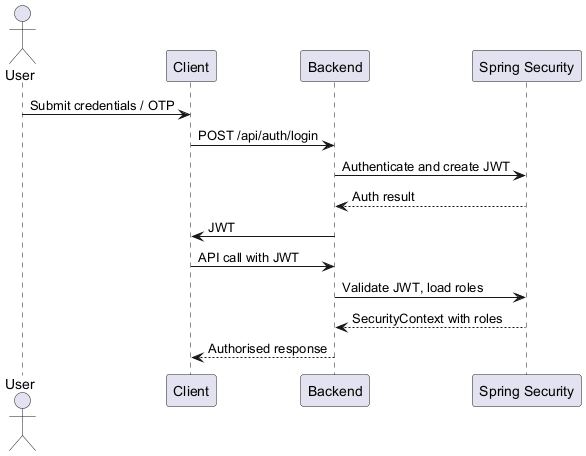
\includegraphics[width=0.9\linewidth]{diagrams/fig_7_9_auth_arch.png}
\caption{Authentication and authorisation flow (backend security architecture).}
\label{fig:backend-auth-arch}
\end{figure}

In relation to Chapter~4, the security architecture addresses the documented reliance on informal communication channels and the associated legal and data-protection uncertainty by introducing authenticated access boundaries (JWT, RBAC, and ownership checks) as default workflow conditions. This is aligned with the identity, trust, and secure-communication requirement domains in Chapter~5 and with RQ3 in Chapter~1.2. At the same time, the unresolved \path{/patientdocuments/**} exposure is retained as an explicit prototype limitation rather than being obscured, so that trust claims remain evidence-aware and proportionate to the current implementation scope.

\section{Quality attributes evaluation}

From a quality-attribute perspective, the current implementation represents a deliberate balance between research-oriented pragmatism and software-engineering rigour. With respect to scalability, the stateless monolith and shared PostgreSQL instance are adequate for the foreseen deployment scale, but they would require either vertical scaling or decomposition into bounded services if the installation were to cover a large national population. Availability is supported through health checks and environment-specific configuration, yet formal service-level objectives and multi-region failover have not been implemented in this iteration.

\textbf{Implementation status.} Implemented in the current prototype: Actuator-based health endpoints, profile-driven environment configuration, and Flyway migrations that support reproducible schema evolution and operational consistency. Partially implemented / currently limited: availability engineering remains at single-service deployment level without formal SLO definitions, redundancy targets, or validated backup/restore runbooks. Planned improvement (future work): define explicit SLOs, formalize and test backup procedures as operational runbooks, and introduce higher-availability deployment patterns where required.

Security benefits from JWT-based role control and ownership checks in service methods, but this remains a prototype-level security baseline rather than a finalized compliance posture. The unresolved document exposure risk and limited security-regression automation are treated as open issues requiring hardening before production use. Performance and maintainability are supported by layered backend structure and established frameworks, while the monolith decision reflects a thesis-stage trade-off: lower integration overhead now, with future decomposition if scale and operational complexity justify it (Bass et al., 2021; Richards \& Ford, 2020). Because no formal benchmark campaign was conducted, the performance discussion remains architectural and explicitly non-empirical.

Methodologically, these quality-attribute trade-offs should be read as part of the thesis design logic rather than as omissions detached from context: the objective was to deliver an implementable and testable backend that can run end-to-end appointments, conversations/messages, documents, tasks, and notifications under realistic project constraints. This positioning is consistent with Chapter~5 requirement priorities and with the research trajectory in Chapter~1.2, where evaluation of usability, acceptability, and perceived impact (RQ4) follows prototype realization. The section therefore frames operational reliability as sufficient for evaluation-readiness, while explicitly deferring production-grade hardening to post-thesis work.

\section{Runtime interaction flows}

To clarify how the components cooperate at runtime, this section sketches four key interaction scenarios as sequence diagrams in PlantUML.

\subsection*{Authentication flow}

\begin{figure}[H]
\centering
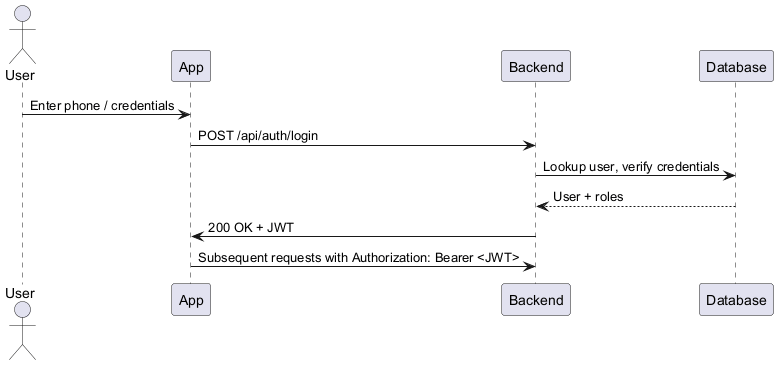
\includegraphics[width=0.9\linewidth]{diagrams/fig_7_5_auth_flow.png}
\caption{Runtime interaction: authentication and JWT issuance.}
\end{figure}

\subsection*{Appointment booking}

\begin{figure}[H]
\centering
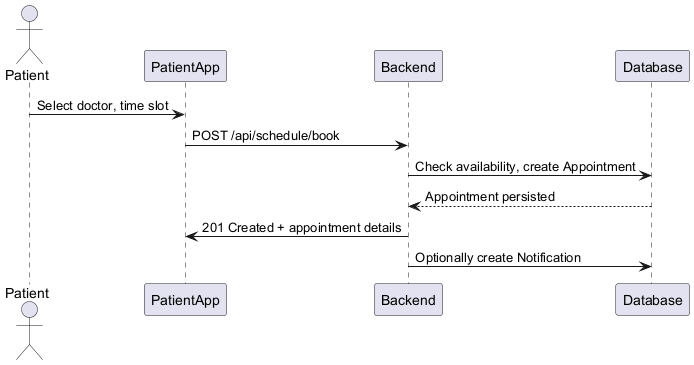
\includegraphics[width=0.9\linewidth]{diagrams/fig_7_6_booking_flow.png}
\caption{Runtime interaction: patient-side appointment booking.}
\end{figure}

\subsection*{Video consultation}

\begin{figure}[H]
\centering
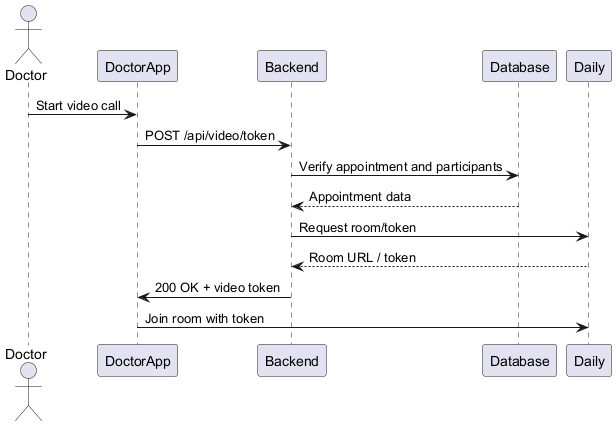
\includegraphics[width=0.9\linewidth]{diagrams/fig_7_7_video_flow.png}
\caption{Runtime interaction: doctor-side video consultation.}
\end{figure}

\subsection*{Document upload and access}

\begin{figure}[H]
\centering
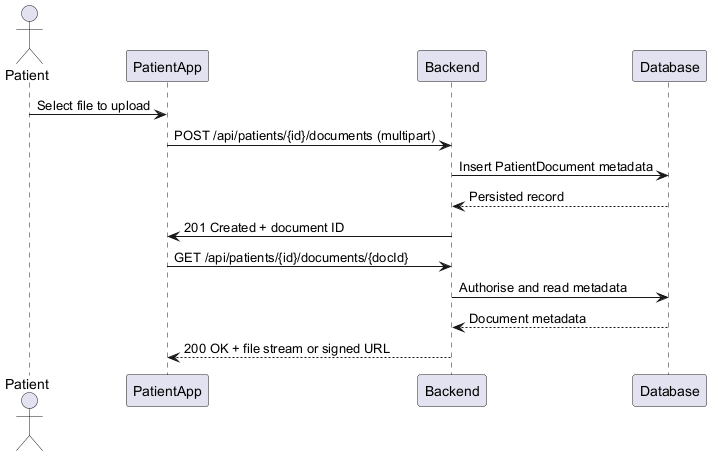
\includegraphics[width=0.9\linewidth]{diagrams/fig_7_8_document_flow.png}
\caption{Runtime interaction: document upload and access.}
\end{figure}

\section{Backend contribution to the research logic}

Methodologically, the backend realizes the transition from qualitative findings to executable service behavior. It operationalizes the requirement classes defined in Chapter~5 and supplies the shared process state consumed by both user interfaces discussed in Chapter~6. This closes the ``needs-to-system'' chain for the server side and prepares the subsequent analysis of client-specific implementation decisions.

\chapter{Doctor Application Implementation}
\label{ch:doctor-implementation}

\section{Role and target users}

The doctor application is the professional-facing interface for clinical workflow execution. It is designed for physicians and administrative users, with emphasis on schedule control, patient context switching, consultation handling, and follow-up coordination. In relation to Chapter~4, this client directly addresses the practical need for structured digital workflows instead of fragmented informal channels, and therefore represents the central operational workspace of the platform.

\section{Technical foundation}

The doctor client is implemented in Flutter. State handling is organized through Riverpod, and navigation combines an app shell pattern with route-based transitions for feature flows. The web deployment target is particularly relevant, including separate hosting contexts for doctor and admin entry points.

\ShifaFigDoctorShell

\section{Architecture rationale and backend interaction}

The choice of Flutter for the doctor-side client reflects a project-specific constraint: one thesis implementation stream had to support rapid iteration of clinically relevant web workflows without building a separate frontend stack. Riverpod was selected to keep dependencies between authentication, appointments, messaging, and notifications explicit as the feature set expanded during implementation. As described by interviewed physicians, the design priority was dependable workflow execution in daily practice rather than UI novelty, so the architecture favors predictable state transitions and backend coherence.

From the doctor client to the backend, all communication is mediated by a small set of HTTP client utilities that encapsulate base URLs, JWT headers, and error-handling conventions. Figure~\ref{fig:doctor-backend-seq} sketches the typical pattern: the web client invokes a REST endpoint, the backend validates the JWT and roles, services consult repositories as needed, and the response is mapped back into domain-specific view models.

\begin{figure}[H]
\centering
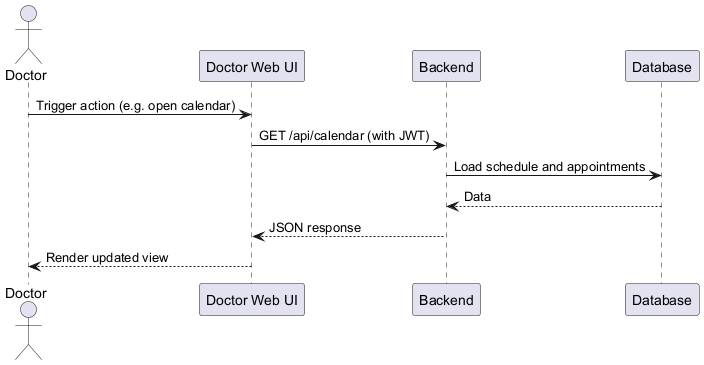
\includegraphics[width=0.9\linewidth]{diagrams/fig_8_1_doctor_seq.png}
\caption{Doctor client interaction with backend.}
\label{fig:doctor-backend-seq}
\end{figure}

\begin{table}[htbp]
\centering
\caption{Representative doctor app dependencies.}
\label{tab:doctor-deps}
\begin{tabularx}{\textwidth}{@{}l>{\RaggedRight\arraybackslash}X@{}}
\toprule
\textbf{Package} & \textbf{Role} \\
\midrule
\texttt{flutter\_riverpod} & State management \\
\texttt{http} & REST client \\
\texttt{table\_calendar}, \texttt{timezone}, \texttt{iana\_time\_zone} & Scheduling and timezone handling \\
\texttt{daily\_flutter} & Video consultation client \\
\texttt{fl\_chart} & Analytics visualization \\
\texttt{cached\_network\_image}, \texttt{record}, \texttt{audioplayers} & Media messaging support \\
\texttt{firebase\_*} & Authentication and push notification integration \\
\bottomrule
\end{tabularx}
\end{table}

\section{Functional structure}

The implemented interface is organized around high-frequency clinical tasks: dashboard/home overview, calendar and availability management, patient list and patient attachment flows, messaging, notifications, tasks, profile management, and appointment/video encounter start flows. Administrative functions are exposed through dedicated admin screens connected to backend admin APIs.

This structure aligns with the requirement narrative in Chapter~5 by emphasizing: secure communication, appointment coordination, and reduced operational friction in daily doctor work. The UI documentation in Chapter~6 shows this progression from wireframes to high-fidelity screens.

\section{Integration with backend services}

The doctor client communicates with backend domains through authenticated HTTP requests. In practical terms, the application consumes appointment, schedule, patient, message, notification, document, and video APIs. For video encounters, session joining is coordinated through backend-issued tokens and the integrated Daily.co stack.

\section{Quality and operational considerations}

The application includes localization support, structured state modules, and error-handling patterns appropriate for production-facing healthcare software. The implementation prioritizes robust task completion (for example, starting appointments, joining calls, and updating schedules) over highly customized visual behavior, consistent with the workflow-centered goals established in Chapters~4 and~5. In this sense, the doctor client can be interpreted as a reliability-oriented execution environment for the requirements mapped in Chapter~5.
\ShifaFigTestBars

\chapter{Patient Application Implementation}
\label{ch:patient-implementation}

\section{Role and user journey}

The patient application provides the citizen-facing entry to the telemedicine process. Its main journey includes onboarding, doctor discovery, booking, appointment review, document access, messaging, and participation in video encounters. This sequence maps directly to the patient-side requirements synthesized in Chapter~5 and illustrated in Chapter~6, and operationalizes the accessibility and trust themes emerging from the interview analysis in Chapter~4.

\section{Technical foundation}

The patient client is implemented in Flutter with GoRouter-based navigation and Riverpod-based state management. The routing model uses tab-preserving navigation for primary areas (home, bookings, documents, doctors) and shell-based navigation for account and supporting modules. This combination preserves usability during repeated appointment and follow-up tasks.

\ShifaFigPatientNav

\section{Architecture rationale and backend interaction}

For the patient app, Flutter was selected to maintain one codebase across Android and iOS under limited development time, while preserving close mapping to the user journeys shown in Chapter~6. GoRouter models tab-preserving navigation and nested flows (for booking and waiting-room transitions), and Riverpod keeps authentication, network, and UI state aligned. This conservative stack is a deliberate scope decision: it reduces platform divergence and handoff friction in core telemedicine tasks, rather than optimizing for feature breadth in the thesis phase.

All patient-facing workflows that modify or retrieve clinical data are backed by REST calls to the backend. The pattern is similar across features: the Flutter app constructs a request with the relevant JWT token, the backend validates authentication and authorisation, services run domain logic and interact with repositories, and the resulting state is serialised back to the app. The following PlantUML snippet captures this for a simplified booking read-flow.

\begin{figure}[H]
\centering
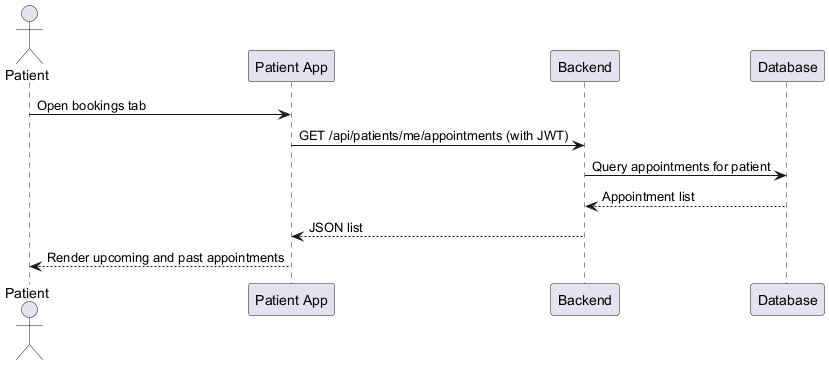
\includegraphics[width=0.9\linewidth]{diagrams/fig_9_1_patient_seq.png}
\caption{Patient client interaction with backend.}
\end{figure}

\begin{table}[htbp]
\centering
\caption{Representative patient app dependencies.}
\label{tab:patient-deps}
\begin{tabularx}{\textwidth}{@{}l>{\RaggedRight\arraybackslash}X@{}}
\toprule
\textbf{Package} & \textbf{Role} \\
\midrule
\texttt{flutter\_riverpod} & State management \\
\texttt{go\_router} & Declarative navigation \\
\texttt{dio} / \texttt{http} & API communication \\
\texttt{firebase\_*} & Auth and notification integration \\
\texttt{daily\_flutter} & Video visit participation \\
\texttt{flutter\_map}, \texttt{geolocator}, \texttt{geocoding} & Location workflows \\
\texttt{local\_auth}, \texttt{flutter\_secure\_storage} & Device-level protection and token storage \\
\texttt{file\_picker}, \texttt{image\_picker} & Document and media uploads \\
\bottomrule
\end{tabularx}
\end{table}

\section{Core modules}

The application is organized into feature modules for authentication, bookings, doctors, documents, chat, notifications, tasks, and profile/settings. Data access is encapsulated in repository classes that consume backend APIs through centralized client configuration. The structure keeps product logic understandable and supports incremental feature evolution.

\section{Experience design and workflow continuity}

From a UX perspective, the patient application prioritizes clarity and stepwise guidance. Appointment and consultation flows are decomposed into explicit stages (selection, confirmation, waiting room, video call, summary), reducing uncertainty for non-technical users. This design approach reflects the usability and trust concerns emerging from the qualitative interviews in Chapter~4.

\section{Deployment and environment handling}

The patient client supports environment-driven backend URL configuration and platform-specific networking behavior for development versus production contexts. In release scenarios, the configuration path prioritizes secure remote endpoints, which supports the privacy and reliability expectations formalized in Chapter~5. Together with the doctor and backend chapters above, this completes the component-level technical argument for the implemented Shifa ecosystem.

\chapter{Security, Quality Attributes, and Operational Considerations}
\label{ch:security-quality}

\section{Security analysis}

The security model of the platform is based on JWT-authenticated requests and role-based authorization. In the implemented prototype, patients and doctors authenticate through Firebase phone OTP steps plus backend-issued JWTs, and administrators use role-gated routes in the doctor web application. Authorization rules in Spring Security map URL patterns (such as \path{/api/patients/me/**}, \path{/api/doctors/me/**}, and \path{/api/admin/**}) to roles, while service-layer methods add resource-level identity checks. This is a practical prototype compromise between security and delivery scope, not a claim that full production-grade token governance is already complete (Kruse et al., 2017; Appari \& Johnson, 2010).

\textbf{Implementation status.} Implemented in the current prototype: OTP + JWT authentication, role-based authorization, and service-level ownership checks on major clinical workflows. Partially implemented / currently limited: document-serving exposure via \path{/patientdocuments/**} remains unresolved in the present codebase, and security-route regression testing is not yet automated in CI. Planned improvement (future work): remove public document exposure by enforcing authenticated download paths and add systematic security test coverage for authorization boundaries.

Two security aspects deserve particular attention from a research perspective. First, document access is currently exposed via a static resource handler for \path{/patientdocuments/**}, with a permissive security rule. This design reflects development expediency but conflicts with the confidentiality requirements articulated in Chapter~5; it should be replaced by controller-mediated access that verifies both role and relationship to the patient record, optionally issuing short-lived signed URLs for temporary access. Second, while the codebase includes building blocks for rate limiting and logging, there is no systematic suite of automated tests that assert security behaviour (for example, distinguishing authorized from unauthorized document access or enforcing role separation on administrative endpoints).

In line with established secure design principles, the future evolution of the system should introduce a test-supported security policy for each route group, extend rate limiting to all high-risk endpoints (authentication and uploads), and treat JWT key management, token lifetimes, and claim validation as explicitly documented design artifacts rather than implicit configuration.

\section{Quality attributes}

From the vantage point of software architecture, the Shifa implementation exhibits specific strengths and limitations across its key quality attributes:

\begin{itemize}[leftmargin=*]
  \item \textbf{Scalability}: the backend monolith is stateless with respect to HTTP sessions and uses PostgreSQL as a single authoritative store. This allows horizontal scaling behind a load balancer, but long-term scalability will be constrained by the database instance and by the lack of explicit bounded contexts for read-heavy versus write-heavy operations.
  \item \textbf{Availability}: health checks and environment-specific configuration provide a foundation for high availability at the current target scale. However, multi-region redundancy and formally specified service-level objectives were not yet in scope, which is acceptable for the thesis context but not sufficient for large-scale national deployment.
  \item \textbf{Security}: the use of JWT and role-based access control, combined with service-layer checks, represents a sound baseline for controlling access to clinical data. The aforementioned static document path and the absence of systematic security tests, however, highlight the importance of continuous hardening.
  \item \textbf{Maintainability}: the modular organization of Flutter feature modules and the layered backend structure support maintainability and incremental evolution. The monolithic backend remains sufficiently small to manage, but its eventual decomposition into separately deployable services would benefit from the existing domain boundaries.
  \item \textbf{Performance}: no formal benchmarking was conducted in the thesis, but the chosen technologies (Spring Boot with JPA; Flutter frontends) are known to deliver adequate performance for the anticipated scale. Performance-critical operations such as document handling and video token issuance are delegated to specialized components, which reduces the likelihood of pure CPU bottlenecks in the core backend.
\end{itemize}

\section{Architectural decisions}

Several architectural decisions can be made explicit in light of established software architecture theory. The choice of Flutter for both clients reflects a ``shared-code'' decision rationale: it reduces implementation and maintenance effort for cross-platform UI while preserving sufficient performance for the interaction patterns described in Chapter~6. The adoption of Spring Boot and Kotlin for the backend reflects a preference for a mature ecosystem, strong typing, and pre-existing integration support for PostgreSQL, security, and observability.

JWT-based authentication was selected to align with RESTful communication and to support stateless client-server interactions, at the cost of additional complexity in token revocation and key management. The decision to implement the backend as a monolith rather than as a set of microservices reflects a deliberate trade-off: it simplifies deployment and diagnostics during early-stage development and empirical evaluation, while leaving the door open to later extraction of domain-specific services once usage patterns and performance profiles are better understood.

\section{Testing and operations}

From an operational viewpoint, the codebase contains concrete deployability hooks (Actuator health endpoints, environment-specific profiles, and Flyway migrations), but testing and CI/CD remain intentionally lean. The backend Railway build currently skips automated tests, and client test coverage is still minimal. This is a known boundary of the thesis artifact: architectural and functional integration were completed first, while full quality gates are explicitly deferred to the post-thesis hardening phase (Humble \& Farley, 2010; Beyer et al., 2016).

\textbf{Implementation status.} Implemented in the current prototype: basic deployability, health observability primitives, and environment-specific configuration. Partially implemented / currently limited: automated test depth is thin and backend test execution is currently skipped in Railway build configuration. Planned improvement (future work): enforce \texttt{./gradlew test}, \texttt{flutter test}, and static analysis gates in CI/CD before deployment promotion.

For a production transition, the following enhancements would be appropriate:

\begin{itemize}[leftmargin=*]
  \item Introduce unit and integration tests for core backend services (authentication, appointments, messaging, documents), including security-focussed tests for authorization boundaries.
  \item Extend Flutter widget tests to cover critical user journeys (login, booking, joining video calls, document access) and to anchor UI regressions.
  \item Establish CI/CD pipelines that enforce static analysis and tests before building and deploying backend and client artifacts, and integrate basic security scanning for dependencies.
  \item Formalize database backup and restore procedures as executable runbooks and exercise them regularly to validate recovery time and recovery point objectives.
\end{itemize}

\section{Implementation status summary}

At the current thesis stage, the implemented prototype already supports end-to-end telemedicine workflows across patient app, doctor app, and backend service: authentication, appointment handling, messaging, document-related interactions, and video-session orchestration. These flows are operational and provide the empirical basis used in Chapters~4--6 and the technical analysis in Chapters~7--11.

At the same time, one security-critical issue remains unresolved and is treated explicitly as open risk: public exposure potential around \path{/patientdocuments/**} under permissive access rules. In addition, the present testing baseline remains limited, and backend tests are currently skipped in Railway build commands. For these reasons, the prototype should not be interpreted as production-grade compliant; it is functionally integrated but still incomplete in security hardening.

Before the July evaluation milestone, the focus is to complete and report evaluation-oriented evidence for usability, trust, and perceived impact, while preserving transparent reporting of implementation limits. Work that remains beyond thesis scope includes production-depth security hardening (including finalized document access redesign and stronger token lifecycle governance), full CI/CD quality gates, formalized backup/recovery operations, and comprehensive machine-readable API contracts.

\chapter{Limitations and Evidence Gaps}

Hosted secrets, Firebase console rules, store pipelines, and penetration tests are out of scope. API tables here omit HTTP verbs per method. UI accessibility was not audited per-widget. Some markdown docs may reference flags not present in code (e.g.\ \texttt{FLAVOR} vs implemented \texttt{ENVIRONMENT} on the patient app).

\textbf{Implementation status.} Implemented in the current prototype: core workflow functionality and chapter-level architectural traceability. Partially implemented / currently limited: compliance-grade evidence for security operations, accessibility, and full API contract completeness. Planned improvement (future work): close these evidence gaps through operational documentation, route-level contract artifacts, and expanded verification pipelines.

\chapter{Future-Oriented Improvements}

\textbf{Status note.} All items in this chapter are planned improvements (future work) and are not claimed as implemented in the current prototype.

\begin{itemize}[leftmargin=*]
  \item Planned improvement (future work): replace public document URLs with authenticated downloads or short-lived signed URLs; remove redundant \texttt{permitAll} exposure.
  \item Planned improvement (future work): publish OpenAPI from controllers or maintain contract tests in CI.
  \item Planned improvement (future work): add integration tests for overlapping patient appointment routes.
  \item Planned improvement (future work): replace stale doctor \path{widget_test.dart}; add backend \path{src/test}; run tests in CI; revisit \texttt{-x test} on Railway.
  \item Planned improvement (future work): add GitHub Actions (or equivalent) for \texttt{flutter analyze}, \texttt{flutter test}, \texttt{./gradlew test}.
  \item Planned improvement (future work): restrict \path{TestDataController} to dev profiles or remove from production images.
\end{itemize}

\chapter{Conclusion}

The Shifa ecosystem delivered in this thesis is best understood as an auditable design-and-implementation artifact: two integrated clients, one backend service, and a reproducible workflow chain grounded in 15 physician interviews and subsequent requirements synthesis. Its strengths are visible in code-level modularization, centralized API access patterns, and coherent cross-client workflow coverage. Its limitations are equally explicit: thin automated testing, skipped backend tests in the Railway build path, no machine-readable published API contract, and unresolved high-severity exposure risk around \path{/patientdocuments/**}. The thesis therefore demonstrates practical system realization under academic constraints, while clearly separating what is implemented now from what remains necessary for production-grade deployment.

\clearpage
\chapter{Literaturverzeichnis}

Bernd Rechel, E. R. (2014). Trends in health systems in the former
Soviet countries. \emph{European Journal of Public Health}.

Ketevan Glonti, B. R. (2013). Health Targets in the Former Soviet
Countries: Responding to the NCD Challenge? \emph{Public Health Reviews,
Vol. 35, No 1}.

The World Bank. (2016). \emph{SYSTEMATIC COUNTRY DIAGNOSTIC for
UZBEKISTAN.} Washington D.C: The World Bank.

World Health Organization. (2022). \emph{Health Systems in Action
Uzbekistan.} World Health Organization.

Mayring, P. (2015). \emph{Qualitative Inhaltsanalyse: Grundlagen und Techniken}
(12., überarbeitete Auflage). Beltz.

Bashshur, R. L., Shannon, G. W., Smith, B. R., Alverson, D. C.,
Antoniotti, N., Barsan, W. G., ... Krupinski, E. A. (2014). The
empirical foundations of telemedicine interventions in primary care.
\emph{Telemedicine and e-Health, 20}(5), 342--375.

Shigekawa, E., Fix, M., Corbett, G., Roby, D. H., \& Coffman, J.
(2018). The current state of telehealth evidence: A rapid review.
\emph{Health Affairs, 37}(12), 1975--1982.

Ekeland, A. G., Bowes, A., \& Flottorp, S. (2010). Effectiveness of
telemedicine: A systematic review of reviews. \emph{International Journal
of Medical Informatics, 79}(11), 736--771.

Venkatesh, V., Morris, M. G., Davis, G. B., \& Davis, F. D. (2003).
User acceptance of information technology: Toward a unified view.
\emph{MIS Quarterly, 27}(3), 425--478.

Greenhalgh, T., Wherton, J., Papoutsi, C., Lynch, J., Hughes, G.,
A'Court, C., ... Shaw, S. (2017). Beyond adoption: A new framework for
theorizing and evaluating nonadoption, abandonment, scale-up, spread, and
sustainability of health and care technologies (NASSS). \emph{Journal of
Medical Internet Research, 19}(11), e367.

Brooke, J. (1996). SUS: A ``quick and dirty'' usability scale. In
P. W. Jordan, B. Thomas, B. A. Weerdmeester, \& I. L. McClelland
(Eds.), \emph{Usability Evaluation in Industry} (pp. 189--194).
Taylor \& Francis.

Nielsen, J. (1994). \emph{Usability Engineering}. Academic Press.

ISO. (2018). \emph{ISO 9241-11:2018 Ergonomics of human-system
interaction---Part 11: Usability: Definitions and concepts}. International
Organization for Standardization.

Maramba, I., Chatterjee, A., \& Newman, C. (2019). Methods of usability
testing in the development of eHealth applications: A scoping review.
\emph{International Journal of Medical Informatics, 126}, 95--104.

Kruse, C. S., Frederick, B., Jacobson, T., \& Monticone, D. K. (2017).
Cybersecurity in healthcare: A systematic review of modern threats and
trends. \emph{Technology and Health Care, 25}(1), 1--10.

Appari, A., \& Johnson, M. E. (2010). Information security and privacy in
healthcare: Current state of research. \emph{International Journal of
Internet and Enterprise Management, 6}(4), 279--314.

Bass, L., Clements, P., \& Kazman, R. (2021). \emph{Software Architecture
in Practice} (4th ed.). Addison-Wesley.

Richards, M., \& Ford, N. (2020). \emph{Fundamentals of Software
Architecture: An Engineering Approach}. O'Reilly Media.

Humble, J., \& Farley, D. (2010). \emph{Continuous Delivery: Reliable
Software Releases through Build, Test, and Deployment Automation}.
Addison-Wesley.

Beyer, B., Jones, C., Petoff, J., \& Murphy, N. R. (Eds.). (2016).
\emph{Site Reliability Engineering: How Google Runs Production Systems}.
O'Reilly Media.

\chapter{Anhang}

Der Anhang enthält ergänzende Materialien, die im Haupttext referenziert
werden, darunter zusätzliche Dokumentations- und Auswertungsunterlagen.
Er dient der Nachvollziehbarkeit, ohne den Fließtext mit ausführlichen
Detailnachweisen zu überladen.

\chapter*{Eidesstattliche Erklärung}
\addcontentsline{toc}{chapter}{Eidesstattliche Erklärung}

Hiermit erkläre ich, dass ich die vorliegende Arbeit selbstständig
verfasst habe, dass ich sie zuvor an keiner anderen Hochschule und in
keinem anderen Studiengang als Prüfungsleistung eingereicht habe und
dass ich keine anderen als die angegebenen Quellen und Hilfsmittel
benutzt habe. Alle Stellen der Arbeit, die wörtlich oder sinngemäß aus
Veröffentlichungen oder aus anderweitigen fremden Äußerungen entnommen
wurden, sind als solche kenntlich gemacht.

Diese Erklärung erfolgt gemäß § 60 Abs. 8 AllgStuPO der Technischen
Universität Berlin.

Ort, Datum Unterschrift



\end{document}
